\documentclass[a4paper]{book}
\usepackage{a4wide}
\usepackage{makeidx}
\usepackage{fancyhdr}
\usepackage{graphicx}
\usepackage{multicol}
\usepackage{float}
\usepackage{textcomp}
\usepackage{alltt}
\usepackage{times}
\usepackage{ifpdf}
\ifpdf
\usepackage[pdftex,
            pagebackref=true,
            colorlinks=true,
            linkcolor=blue,
            unicode
           ]{hyperref}
\else
\usepackage[ps2pdf,
            pagebackref=true,
            colorlinks=true,
            linkcolor=blue,
            unicode
           ]{hyperref}
\usepackage{pspicture}
\fi
\usepackage[utf8]{inputenc}
\usepackage{doxygen}
\makeindex
\setcounter{tocdepth}{1}
\renewcommand{\footrulewidth}{0.4pt}
\begin{document}
\begin{titlepage}
\vspace*{7cm}
\begin{center}
{\Large ACO-R \\[1ex]\large 1 }\\
\vspace*{1cm}
{\large Generated by Doxygen 1.5.5}\\
\vspace*{0.5cm}
{\small Wed Feb 4 11:12:19 2009}\\
\end{center}
\end{titlepage}
\clearemptydoublepage
\pagenumbering{roman}
\tableofcontents
\clearemptydoublepage
\pagenumbering{arabic}
\chapter{Class Index}
\section{Class Hierarchy}
This inheritance list is sorted roughly, but not completely, alphabetically:\begin{CompactList}
\item \contentsline{section}{pso::\_\-object}{\pageref{classpso_1_1__object}}{}
\begin{CompactList}
\item \contentsline{section}{pso::Function}{\pageref{classpso_1_1Function}}{}
\begin{CompactList}
\item \contentsline{section}{pso::Ackley}{\pageref{classpso_1_1Ackley}}{}
\begin{CompactList}
\item \contentsline{section}{pso::AckleyPtr}{\pageref{classpso_1_1AckleyPtr}}{}
\end{CompactList}
\item \contentsline{section}{pso::Freudenstein}{\pageref{classpso_1_1Freudenstein}}{}
\begin{CompactList}
\item \contentsline{section}{pso::FreudensteinPtr}{\pageref{classpso_1_1FreudensteinPtr}}{}
\end{CompactList}
\item \contentsline{section}{pso::FunctionPtr}{\pageref{classpso_1_1FunctionPtr}}{}
\item \contentsline{section}{pso::Griewank}{\pageref{classpso_1_1Griewank}}{}
\begin{CompactList}
\item \contentsline{section}{pso::GriewankPtr}{\pageref{classpso_1_1GriewankPtr}}{}
\end{CompactList}
\item \contentsline{section}{pso::Levy5}{\pageref{classpso_1_1Levy5}}{}
\begin{CompactList}
\item \contentsline{section}{pso::Levy5Ptr}{\pageref{classpso_1_1Levy5Ptr}}{}
\end{CompactList}
\item \contentsline{section}{pso::MovingGoal}{\pageref{classpso_1_1MovingGoal}}{}
\begin{CompactList}
\item \contentsline{section}{pso::MovingGoalPtr}{\pageref{classpso_1_1MovingGoalPtr}}{}
\end{CompactList}
\item \contentsline{section}{pso::MovingPeaks}{\pageref{classpso_1_1MovingPeaks}}{}
\begin{CompactList}
\item \contentsline{section}{pso::MovingPeaksPtr}{\pageref{classpso_1_1MovingPeaksPtr}}{}
\end{CompactList}
\item \contentsline{section}{pso::Quadric}{\pageref{classpso_1_1Quadric}}{}
\begin{CompactList}
\item \contentsline{section}{pso::QuadricPtr}{\pageref{classpso_1_1QuadricPtr}}{}
\end{CompactList}
\item \contentsline{section}{pso::Rastrigin}{\pageref{classpso_1_1Rastrigin}}{}
\begin{CompactList}
\item \contentsline{section}{pso::RastriginPtr}{\pageref{classpso_1_1RastriginPtr}}{}
\end{CompactList}
\item \contentsline{section}{pso::Rosenbrock}{\pageref{classpso_1_1Rosenbrock}}{}
\begin{CompactList}
\item \contentsline{section}{pso::RosenbrockPtr}{\pageref{classpso_1_1RosenbrockPtr}}{}
\end{CompactList}
\item \contentsline{section}{pso::Schaffer}{\pageref{classpso_1_1Schaffer}}{}
\begin{CompactList}
\item \contentsline{section}{pso::SchafferPtr}{\pageref{classpso_1_1SchafferPtr}}{}
\end{CompactList}
\item \contentsline{section}{pso::Schwefel}{\pageref{classpso_1_1Schwefel}}{}
\begin{CompactList}
\item \contentsline{section}{pso::SchwefelPtr}{\pageref{classpso_1_1SchwefelPtr}}{}
\end{CompactList}
\item \contentsline{section}{pso::Sinusoidal}{\pageref{classpso_1_1Sinusoidal}}{}
\begin{CompactList}
\item \contentsline{section}{pso::SinusoidalPtr}{\pageref{classpso_1_1SinusoidalPtr}}{}
\end{CompactList}
\item \contentsline{section}{pso::Sphere}{\pageref{classpso_1_1Sphere}}{}
\begin{CompactList}
\item \contentsline{section}{pso::SpherePtr}{\pageref{classpso_1_1SpherePtr}}{}
\end{CompactList}
\end{CompactList}
\item \contentsline{section}{pso::PSO}{\pageref{classpso_1_1PSO}}{}
\begin{CompactList}
\item \contentsline{section}{pso::PSOPtr}{\pageref{classpso_1_1PSOPtr}}{}
\end{CompactList}
\item \contentsline{section}{pso::PsoStatistics}{\pageref{classpso_1_1PsoStatistics}}{}
\begin{CompactList}
\item \contentsline{section}{pso::PsoStatisticsPtr}{\pageref{classpso_1_1PsoStatisticsPtr}}{}
\end{CompactList}
\end{CompactList}
\item \contentsline{section}{Bird}{\pageref{classBird}}{}
\item \contentsline{section}{BirdContainer}{\pageref{structBirdContainer}}{}
\item \contentsline{section}{displayGraph::editParameters}{\pageref{classdisplayGraph_1_1editParameters}}{}
\item \contentsline{section}{Function}{\pageref{classFunction}}{}
\begin{CompactList}
\item \contentsline{section}{Ackley}{\pageref{classAckley}}{}
\item \contentsline{section}{Freudenstein}{\pageref{classFreudenstein}}{}
\item \contentsline{section}{Griewank}{\pageref{classGriewank}}{}
\item \contentsline{section}{Levy5}{\pageref{classLevy5}}{}
\item \contentsline{section}{MovingGoal}{\pageref{classMovingGoal}}{}
\item \contentsline{section}{MovingPeaks}{\pageref{classMovingPeaks}}{}
\item \contentsline{section}{Quadric}{\pageref{classQuadric}}{}
\item \contentsline{section}{Rastrigin}{\pageref{classRastrigin}}{}
\item \contentsline{section}{Rosenbrock}{\pageref{classRosenbrock}}{}
\item \contentsline{section}{Schaffer}{\pageref{classSchaffer}}{}
\item \contentsline{section}{Schwefel}{\pageref{classSchwefel}}{}
\item \contentsline{section}{Sinusoidal}{\pageref{classSinusoidal}}{}
\item \contentsline{section}{Sphere}{\pageref{classSphere}}{}
\item \contentsline{section}{Zitzler3}{\pageref{classZitzler3}}{}
\end{CompactList}
\item \contentsline{section}{displayGraph::GraphDisplay}{\pageref{classdisplayGraph_1_1GraphDisplay}}{}
\item \contentsline{section}{paramWindow::ParameterWindow}{\pageref{classparamWindow_1_1ParameterWindow}}{}
\item \contentsline{section}{paramWindow::ParameterWindow\_\-new}{\pageref{classparamWindow_1_1ParameterWindow__new}}{}
\item \contentsline{section}{PSO}{\pageref{classPSO}}{}
\begin{CompactList}
\item \contentsline{section}{LSearch}{\pageref{classLSearch}}{}
\end{CompactList}
\item \contentsline{section}{psoParameter-old::PsoParameter}{\pageref{classpsoParameter-old_1_1PsoParameter}}{}
\item \contentsline{section}{psoParameter::PsoParameter}{\pageref{classpsoParameter_1_1PsoParameter}}{}
\item \contentsline{section}{psoParameter::PsoParameter2}{\pageref{classpsoParameter_1_1PsoParameter2}}{}
\item \contentsline{section}{psoParameter::PsoParameter3}{\pageref{classpsoParameter_1_1PsoParameter3}}{}
\item \contentsline{section}{PsoStatistics}{\pageref{classPsoStatistics}}{}
\item \contentsline{section}{PySwigObject}{\pageref{structPySwigObject}}{}
\item \contentsline{section}{PySwigPacked}{\pageref{structPySwigPacked}}{}
\item \contentsline{section}{SequenceGenerator}{\pageref{classSequenceGenerator}}{}
\item \contentsline{section}{displayGraph::showDescription}{\pageref{classdisplayGraph_1_1showDescription}}{}
\item \contentsline{section}{Swarm}{\pageref{classSwarm}}{}
\begin{CompactList}
\item \contentsline{section}{LocalSwarm}{\pageref{classLocalSwarm}}{}
\item \contentsline{section}{PyramidSwarm}{\pageref{classPyramidSwarm}}{}
\begin{CompactList}
\item \contentsline{section}{AdaptivePyramidSwarm}{\pageref{classAdaptivePyramidSwarm}}{}
\item \contentsline{section}{DynamicPyramidSwarm}{\pageref{classDynamicPyramidSwarm}}{}
\end{CompactList}
\item \contentsline{section}{RingSwarm}{\pageref{classRingSwarm}}{}
\item \contentsline{section}{ScoutSwarm}{\pageref{classScoutSwarm}}{}
\end{CompactList}
\item \contentsline{section}{swig\_\-const\_\-info}{\pageref{structswig__const__info}}{}
\item \contentsline{section}{swig\_\-globalvar}{\pageref{structswig__globalvar}}{}
\item \contentsline{section}{swig\_\-type\_\-info}{\pageref{structswig__type__info}}{}
\item \contentsline{section}{swig\_\-varlinkobject}{\pageref{structswig__varlinkobject}}{}
\item \contentsline{section}{tree$<$ T, tree\_\-node\_\-allocator $>$}{\pageref{classtree}}{}
\item \contentsline{section}{tree$<$ T, tree\_\-node\_\-allocator $>$::compare\_\-nodes$<$ StrictWeakOrdering $>$}{\pageref{classtree_1_1compare__nodes}}{}
\item \contentsline{section}{tree$<$ T, tree\_\-node\_\-allocator $>$::iterator\_\-base}{\pageref{classtree_1_1iterator__base}}{}
\begin{CompactList}
\item \contentsline{section}{tree$<$ T, tree\_\-node\_\-allocator $>$::fixed\_\-depth\_\-iterator}{\pageref{classtree_1_1fixed__depth__iterator}}{}
\item \contentsline{section}{tree$<$ T, tree\_\-node\_\-allocator $>$::post\_\-order\_\-iterator}{\pageref{classtree_1_1post__order__iterator}}{}
\item \contentsline{section}{tree$<$ T, tree\_\-node\_\-allocator $>$::pre\_\-order\_\-iterator}{\pageref{classtree_1_1pre__order__iterator}}{}
\item \contentsline{section}{tree$<$ T, tree\_\-node\_\-allocator $>$::sibling\_\-iterator}{\pageref{classtree_1_1sibling__iterator}}{}
\end{CompactList}
\item \contentsline{section}{tree$<$ T, tree\_\-node\_\-allocator $>$::iterator\_\-base\_\-less}{\pageref{classtree_1_1iterator__base__less}}{}
\item \contentsline{section}{tree\_\-node\_\-$<$ T $>$}{\pageref{classtree__node__}}{}
\end{CompactList}

\chapter{Class Index}
\section{Class List}
Here are the classes, structs, unions and interfaces with brief descriptions:\begin{CompactList}
\item\contentsline{section}{\hyperlink{classAckley}{Ackley} }{\pageref{classAckley}}{}
\item\contentsline{section}{\hyperlink{classColony}{Colony} }{\pageref{classColony}}{}
\item\contentsline{section}{\hyperlink{classFunction}{Function} }{\pageref{classFunction}}{}
\item\contentsline{section}{\hyperlink{classGriewank}{Griewank} }{\pageref{classGriewank}}{}
\item\contentsline{section}{\hyperlink{classRandom}{Random} }{\pageref{classRandom}}{}
\item\contentsline{section}{\hyperlink{classRastrigin}{Rastrigin} }{\pageref{classRastrigin}}{}
\item\contentsline{section}{\hyperlink{classSolution}{Solution} }{\pageref{classSolution}}{}
\item\contentsline{section}{\hyperlink{classTimer}{Timer} }{\pageref{classTimer}}{}
\end{CompactList}

\chapter{File Index}
\section{File List}
Here is a list of all files with brief descriptions:\begin{CompactList}
\item\contentsline{section}{\hyperlink{aco-r_8cpp}{aco-r.cpp} }{\pageref{aco-r_8cpp}}{}
\item\contentsline{section}{\hyperlink{Colony_8cpp}{Colony.cpp} }{\pageref{Colony_8cpp}}{}
\item\contentsline{section}{\hyperlink{Colony_8h}{Colony.h} }{\pageref{Colony_8h}}{}
\item\contentsline{section}{\hyperlink{config_8h}{config.h} }{\pageref{config_8h}}{}
\item\contentsline{section}{\hyperlink{Functions_8cpp}{Functions.cpp} }{\pageref{Functions_8cpp}}{}
\item\contentsline{section}{\hyperlink{Functions_8h}{Functions.h} }{\pageref{Functions_8h}}{}
\item\contentsline{section}{\hyperlink{Random_8cc}{Random.cc} }{\pageref{Random_8cc}}{}
\item\contentsline{section}{\hyperlink{Random_8h}{Random.h} }{\pageref{Random_8h}}{}
\item\contentsline{section}{\hyperlink{Solution_8cpp}{Solution.cpp} }{\pageref{Solution_8cpp}}{}
\item\contentsline{section}{\hyperlink{Solution_8h}{Solution.h} }{\pageref{Solution_8h}}{}
\item\contentsline{section}{\hyperlink{Timer_8cc}{Timer.cc} }{\pageref{Timer_8cc}}{}
\item\contentsline{section}{\hyperlink{Timer_8h}{Timer.h} }{\pageref{Timer_8h}}{}
\end{CompactList}

\chapter{Class Documentation}
\hypertarget{classAckley}{
\section{Ackley Class Reference}
\label{classAckley}\index{Ackley@{Ackley}}
}
The \hyperlink{classAckley}{Ackley} function.  


{\tt \#include $<$optfunctions.h$>$}

Inheritance diagram for Ackley:Collaboration diagram for Ackley:\subsection*{Public Member Functions}
\begin{CompactItemize}
\item 
\hyperlink{classAckley_92a07ab7c3d1cbc6914c20598d304e78}{Ackley} (int n, \hyperlink{optfunctions_8h_ae9aa3a5dd199a43e77abc2cccf4477e}{dynamicStyle\_\-type} dynamicStyle\_\-in)
\begin{CompactList}\small\item\em Constructor with dimension n. \item\end{CompactList}\item 
\hyperlink{classAckley_744516ce25ffab41b589b7d39a52c380}{$\sim$Ackley} ()
\begin{CompactList}\small\item\em The allocated ressources are freed. \item\end{CompactList}\item 
double \hyperlink{classAckley_bfd43046b591f73cf05527333220b5e2}{evaluate} (const vector$<$ double $>$ \&pos)
\begin{CompactList}\small\item\em The evaluation function f(pos). \item\end{CompactList}\end{CompactItemize}


\subsection{Detailed Description}
The \hyperlink{classAckley}{Ackley} function. 

\subsection{Constructor \& Destructor Documentation}
\hypertarget{classAckley_92a07ab7c3d1cbc6914c20598d304e78}{
\index{Ackley@{Ackley}!Ackley@{Ackley}}
\index{Ackley@{Ackley}!Ackley@{Ackley}}
\subsubsection{\setlength{\rightskip}{0pt plus 5cm}Ackley::Ackley (int {\em n}, \/  {\bf dynamicStyle\_\-type} {\em dynamicStyle\_\-in})}}
\label{classAckley_92a07ab7c3d1cbc6914c20598d304e78}


Constructor with dimension n. 

\hypertarget{classAckley_744516ce25ffab41b589b7d39a52c380}{
\index{Ackley@{Ackley}!$\sim$Ackley@{$\sim$Ackley}}
\index{$\sim$Ackley@{$\sim$Ackley}!Ackley@{Ackley}}
\subsubsection{\setlength{\rightskip}{0pt plus 5cm}Ackley::$\sim$Ackley ()}}
\label{classAckley_744516ce25ffab41b589b7d39a52c380}


The allocated ressources are freed. 



\subsection{Member Function Documentation}
\hypertarget{classAckley_bfd43046b591f73cf05527333220b5e2}{
\index{Ackley@{Ackley}!evaluate@{evaluate}}
\index{evaluate@{evaluate}!Ackley@{Ackley}}
\subsubsection{\setlength{\rightskip}{0pt plus 5cm}double Ackley::evaluate (const vector$<$ double $>$ \& {\em pos})\hspace{0.3cm}{\tt  \mbox{[}virtual\mbox{]}}}}
\label{classAckley_bfd43046b591f73cf05527333220b5e2}


The evaluation function f(pos). 



Reimplemented from \hyperlink{classFunction_159260a1fc3afa8932491e4057b6b844}{Function}.

The documentation for this class was generated from the following files:\begin{CompactItemize}
\item 
/home/andrej/workspace/hpso/pso\_\-src/\hyperlink{optfunctions_8h}{optfunctions.h}\item 
/home/andrej/workspace/hpso/pso\_\-src/\hyperlink{optfunctions_8cpp}{optfunctions.cpp}\end{CompactItemize}

\hypertarget{classColony}{
\section{Colony Class Reference}
\label{classColony}\index{Colony@{Colony}}
}
{\tt \#include $<$Colony.h$>$}

Collaboration diagram for Colony:\nopagebreak
\begin{figure}[H]
\begin{center}
\leavevmode
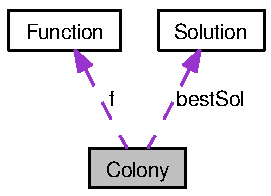
\includegraphics[width=83pt]{classColony__coll__graph}
\end{center}
\end{figure}
\subsection*{Public Member Functions}
\begin{CompactItemize}
\item 
\hyperlink{classColony_af760edad97dee7263b86913d3bb4f98}{Colony} ()
\item 
\hyperlink{classColony_13871283edd253b794363e33a8920f6b}{Colony} (\hyperlink{classFunction}{Function} $\ast$my\_\-f, int my\_\-archive\_\-size, int my\_\-n\_\-of\_\-ants, double my\_\-q, double my\_\-rho)
\item 
\hyperlink{classColony_9cebe4a25260c8da7c99d10b0dab5a4e}{$\sim$Colony} ()
\item 
int \hyperlink{classColony_c46a39e897255d72662ed9b1677bc91a}{initialize} ()
\item 
int \hyperlink{classColony_81a0f7680e31680188f40f5293510711}{iterate} ()
\item 
void \hyperlink{classColony_ca86ca3a2dcad9f2e98edfb449c6bbe2}{delete\_\-worst} ()
\item 
double \hyperlink{classColony_392a128abc861f658f92aa98f6c21585}{gaussian} (double mean, double var)
\end{CompactItemize}
\subsection*{Public Attributes}
\begin{CompactItemize}
\item 
\hyperlink{classFunction}{Function} $\ast$ \hyperlink{classColony_bf5614747e9e944cd2af6ffa83e3cf38}{f}
\item 
\hyperlink{classSolution}{Solution} $\ast$ \hyperlink{classColony_3030d0a11898b83414df4a3f8878c141}{bestSol}
\item 
int \hyperlink{classColony_6ab1bba15c25d8c2e38e2a3632d63661}{archive\_\-size}
\item 
int \hyperlink{classColony_5398847209293075291ecec0c242b19e}{n\_\-of\_\-ants}
\item 
double \hyperlink{classColony_34885da4424133c87e8c887ea9b26f14}{q}
\item 
double \hyperlink{classColony_49231f75985e7ba471f22438e5449714}{rho}
\item 
list$<$ \hyperlink{classSolution}{Solution} $\ast$ $>$ \hyperlink{classColony_74323b8c562a6e02b786be593a6ad25b}{archive}
\item 
int \hyperlink{classColony_f6d58daa2f800a0c086c43ff0a8d49d0}{nonimpr\_\-counter}
\end{CompactItemize}


\subsection{Constructor \& Destructor Documentation}
\hypertarget{classColony_af760edad97dee7263b86913d3bb4f98}{
\index{Colony@{Colony}!Colony@{Colony}}
\index{Colony@{Colony}!Colony@{Colony}}
\subsubsection{\setlength{\rightskip}{0pt plus 5cm}Colony::Colony ()}}
\label{classColony_af760edad97dee7263b86913d3bb4f98}


\hypertarget{classColony_13871283edd253b794363e33a8920f6b}{
\index{Colony@{Colony}!Colony@{Colony}}
\index{Colony@{Colony}!Colony@{Colony}}
\subsubsection{\setlength{\rightskip}{0pt plus 5cm}Colony::Colony ({\bf Function} $\ast$ {\em my\_\-f}, \/  int {\em my\_\-archive\_\-size}, \/  int {\em my\_\-n\_\-of\_\-ants}, \/  double {\em my\_\-q}, \/  double {\em my\_\-rho})}}
\label{classColony_13871283edd253b794363e33a8920f6b}


\hypertarget{classColony_9cebe4a25260c8da7c99d10b0dab5a4e}{
\index{Colony@{Colony}!$\sim$Colony@{$\sim$Colony}}
\index{$\sim$Colony@{$\sim$Colony}!Colony@{Colony}}
\subsubsection{\setlength{\rightskip}{0pt plus 5cm}Colony::$\sim$Colony ()}}
\label{classColony_9cebe4a25260c8da7c99d10b0dab5a4e}




\subsection{Member Function Documentation}
\hypertarget{classColony_c46a39e897255d72662ed9b1677bc91a}{
\index{Colony@{Colony}!initialize@{initialize}}
\index{initialize@{initialize}!Colony@{Colony}}
\subsubsection{\setlength{\rightskip}{0pt plus 5cm}int Colony::initialize ()}}
\label{classColony_c46a39e897255d72662ed9b1677bc91a}




Here is the call graph for this function:\nopagebreak
\begin{figure}[H]
\begin{center}
\leavevmode
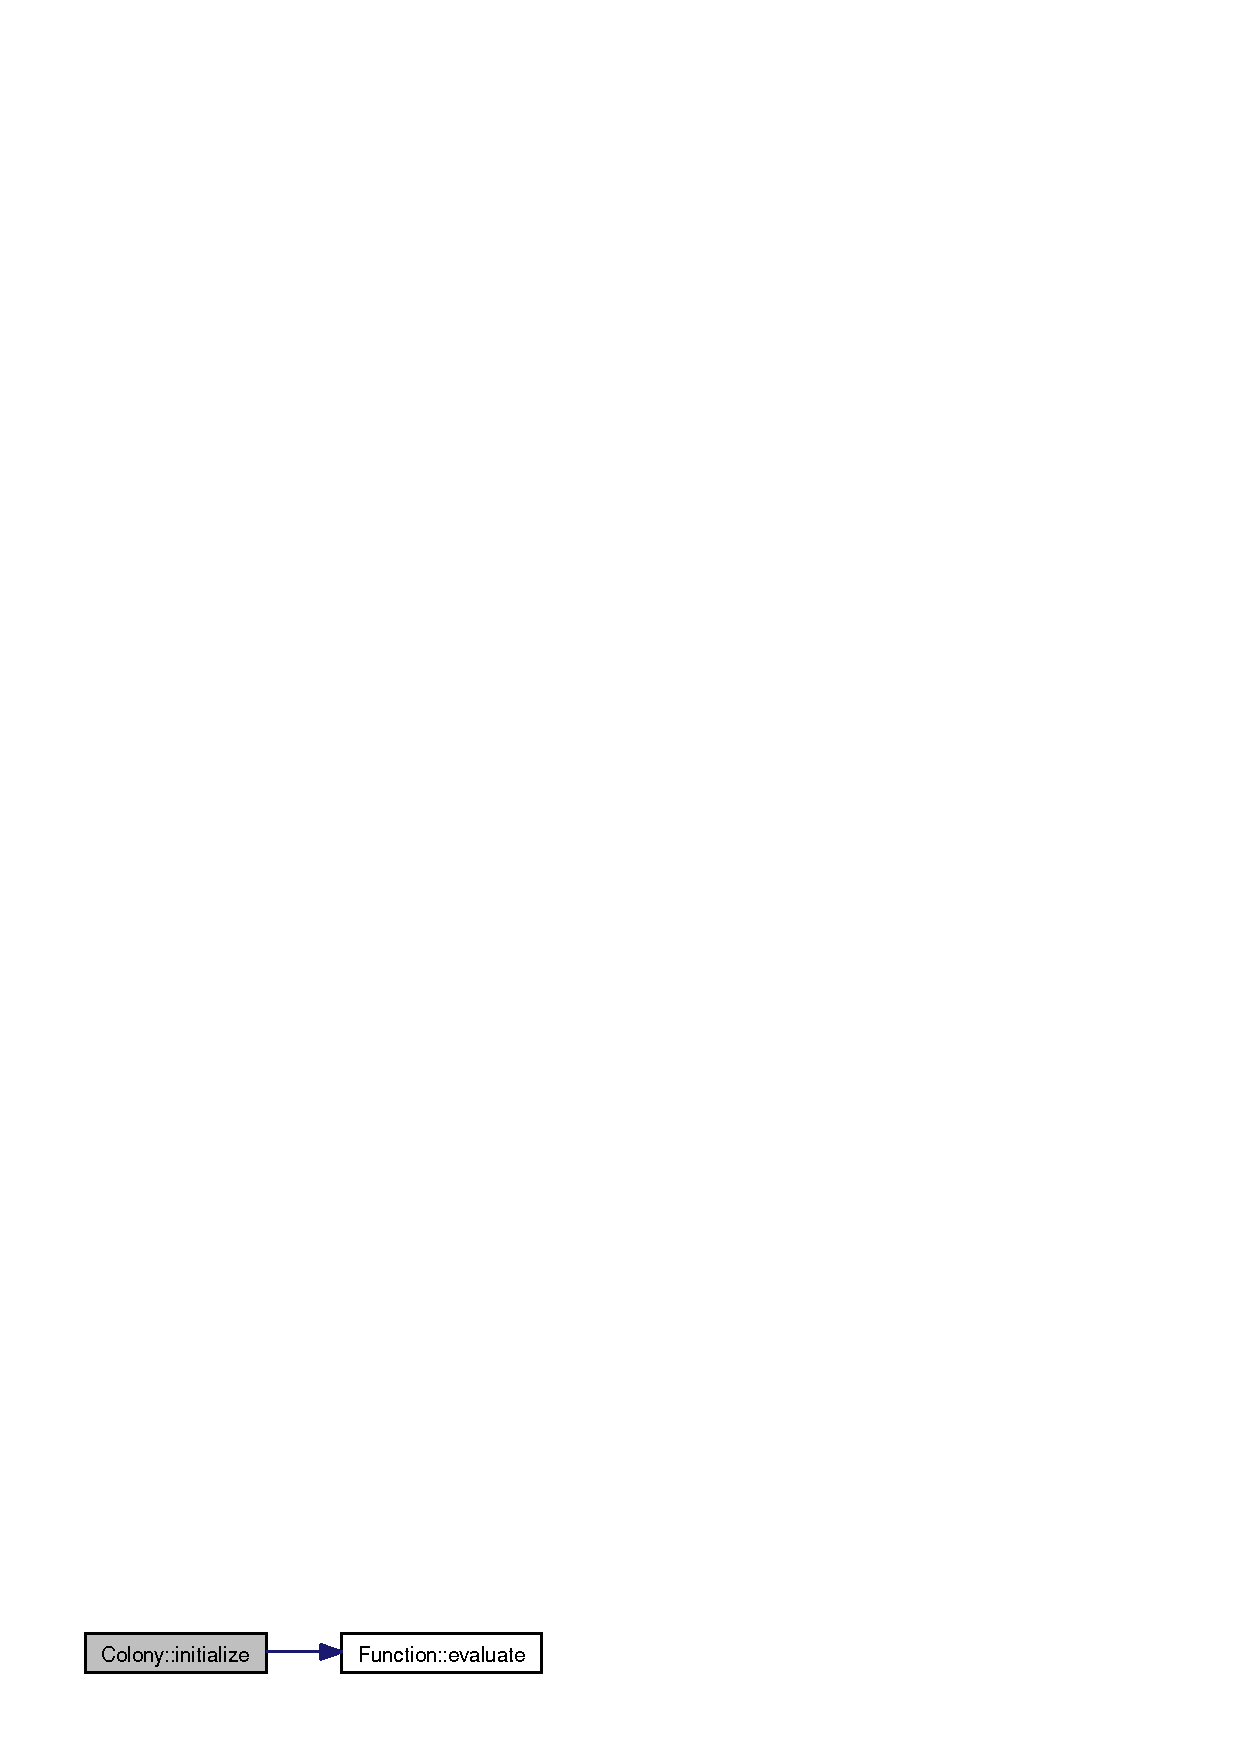
\includegraphics[width=132pt]{classColony_c46a39e897255d72662ed9b1677bc91a_cgraph}
\end{center}
\end{figure}
\hypertarget{classColony_81a0f7680e31680188f40f5293510711}{
\index{Colony@{Colony}!iterate@{iterate}}
\index{iterate@{iterate}!Colony@{Colony}}
\subsubsection{\setlength{\rightskip}{0pt plus 5cm}int Colony::iterate ()}}
\label{classColony_81a0f7680e31680188f40f5293510711}




Here is the call graph for this function:\nopagebreak
\begin{figure}[H]
\begin{center}
\leavevmode
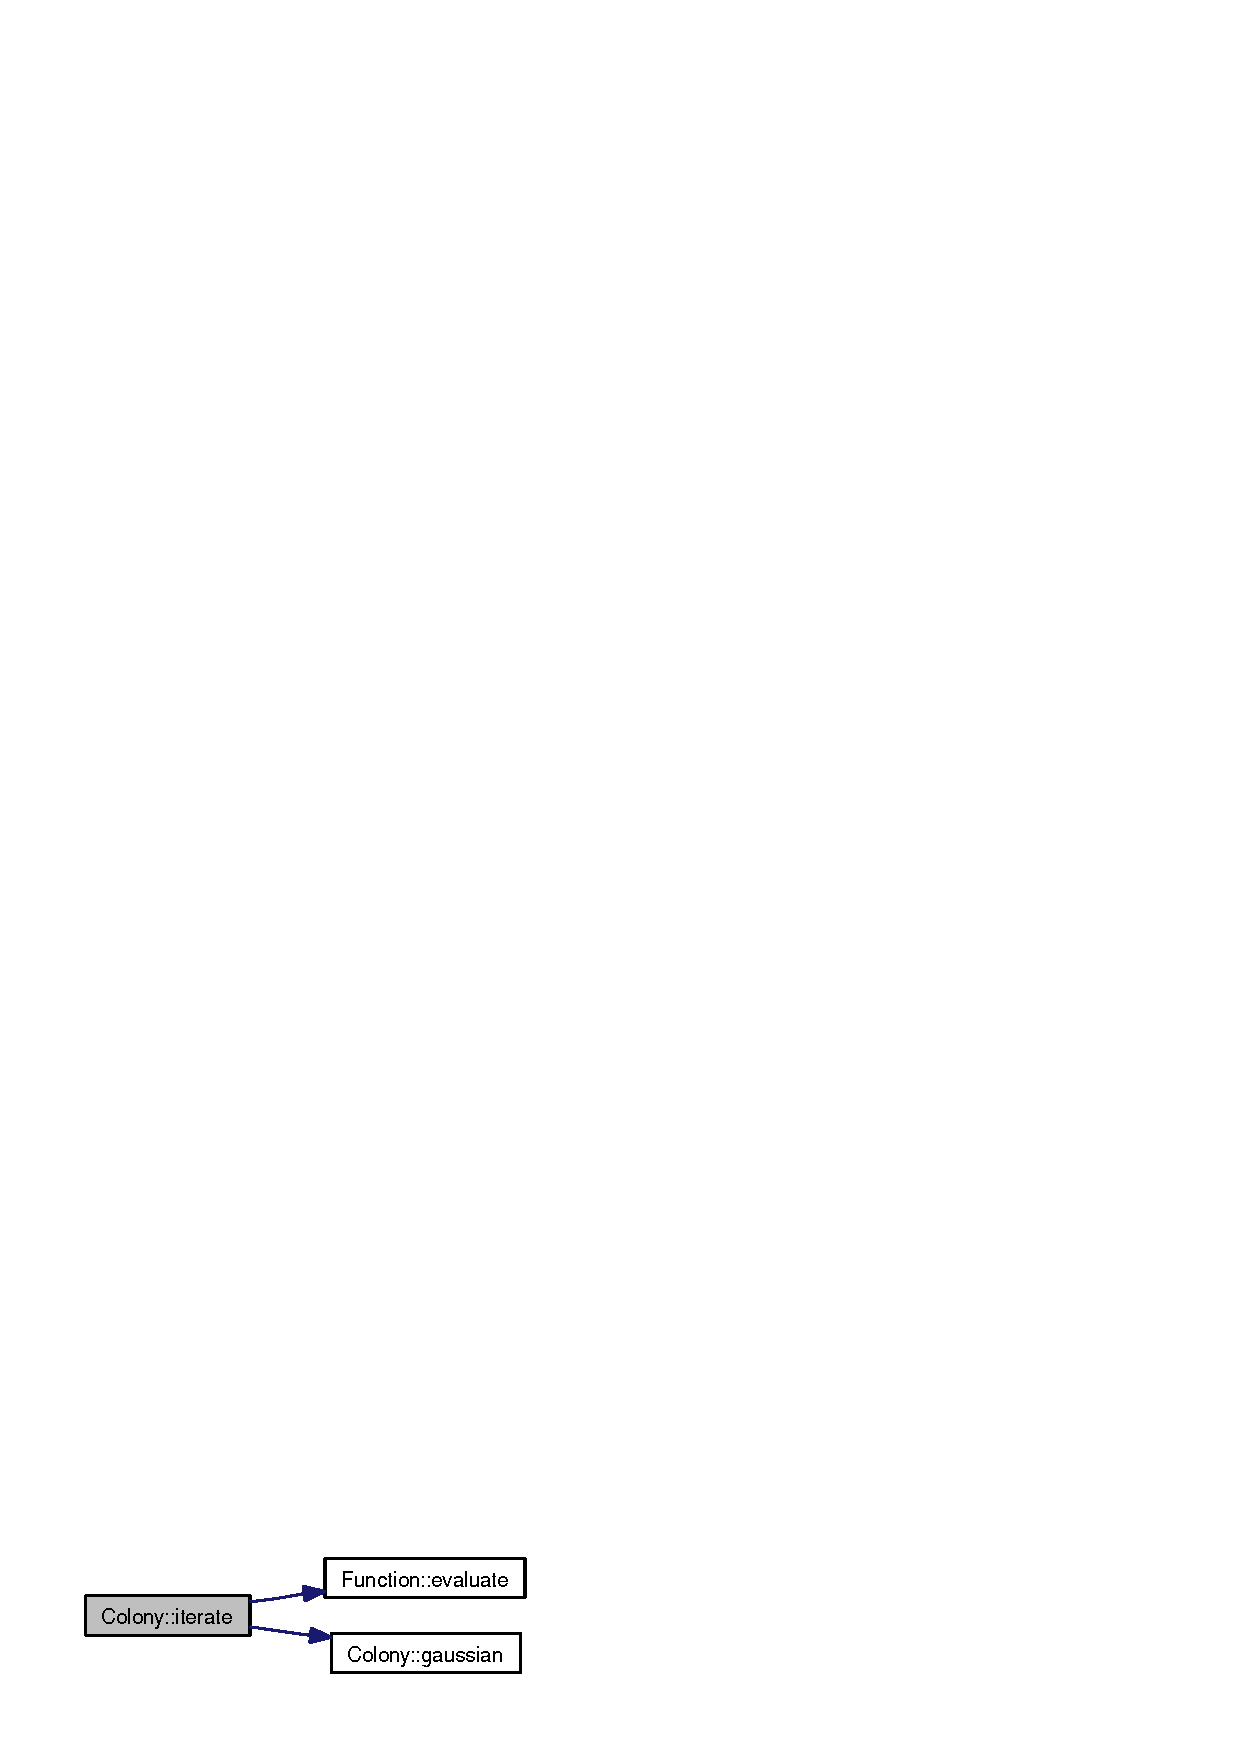
\includegraphics[width=128pt]{classColony_81a0f7680e31680188f40f5293510711_cgraph}
\end{center}
\end{figure}
\hypertarget{classColony_ca86ca3a2dcad9f2e98edfb449c6bbe2}{
\index{Colony@{Colony}!delete\_\-worst@{delete\_\-worst}}
\index{delete\_\-worst@{delete\_\-worst}!Colony@{Colony}}
\subsubsection{\setlength{\rightskip}{0pt plus 5cm}void Colony::delete\_\-worst ()}}
\label{classColony_ca86ca3a2dcad9f2e98edfb449c6bbe2}


\hypertarget{classColony_392a128abc861f658f92aa98f6c21585}{
\index{Colony@{Colony}!gaussian@{gaussian}}
\index{gaussian@{gaussian}!Colony@{Colony}}
\subsubsection{\setlength{\rightskip}{0pt plus 5cm}double Colony::gaussian (double {\em mean}, \/  double {\em var})}}
\label{classColony_392a128abc861f658f92aa98f6c21585}




\subsection{Member Data Documentation}
\hypertarget{classColony_bf5614747e9e944cd2af6ffa83e3cf38}{
\index{Colony@{Colony}!f@{f}}
\index{f@{f}!Colony@{Colony}}
\subsubsection{\setlength{\rightskip}{0pt plus 5cm}{\bf Function}$\ast$ {\bf Colony::f}}}
\label{classColony_bf5614747e9e944cd2af6ffa83e3cf38}


\hypertarget{classColony_3030d0a11898b83414df4a3f8878c141}{
\index{Colony@{Colony}!bestSol@{bestSol}}
\index{bestSol@{bestSol}!Colony@{Colony}}
\subsubsection{\setlength{\rightskip}{0pt plus 5cm}{\bf Solution}$\ast$ {\bf Colony::bestSol}}}
\label{classColony_3030d0a11898b83414df4a3f8878c141}


\hypertarget{classColony_6ab1bba15c25d8c2e38e2a3632d63661}{
\index{Colony@{Colony}!archive\_\-size@{archive\_\-size}}
\index{archive\_\-size@{archive\_\-size}!Colony@{Colony}}
\subsubsection{\setlength{\rightskip}{0pt plus 5cm}int {\bf Colony::archive\_\-size}}}
\label{classColony_6ab1bba15c25d8c2e38e2a3632d63661}


\hypertarget{classColony_5398847209293075291ecec0c242b19e}{
\index{Colony@{Colony}!n\_\-of\_\-ants@{n\_\-of\_\-ants}}
\index{n\_\-of\_\-ants@{n\_\-of\_\-ants}!Colony@{Colony}}
\subsubsection{\setlength{\rightskip}{0pt plus 5cm}int {\bf Colony::n\_\-of\_\-ants}}}
\label{classColony_5398847209293075291ecec0c242b19e}


\hypertarget{classColony_34885da4424133c87e8c887ea9b26f14}{
\index{Colony@{Colony}!q@{q}}
\index{q@{q}!Colony@{Colony}}
\subsubsection{\setlength{\rightskip}{0pt plus 5cm}double {\bf Colony::q}}}
\label{classColony_34885da4424133c87e8c887ea9b26f14}


\hypertarget{classColony_49231f75985e7ba471f22438e5449714}{
\index{Colony@{Colony}!rho@{rho}}
\index{rho@{rho}!Colony@{Colony}}
\subsubsection{\setlength{\rightskip}{0pt plus 5cm}double {\bf Colony::rho}}}
\label{classColony_49231f75985e7ba471f22438e5449714}


\hypertarget{classColony_74323b8c562a6e02b786be593a6ad25b}{
\index{Colony@{Colony}!archive@{archive}}
\index{archive@{archive}!Colony@{Colony}}
\subsubsection{\setlength{\rightskip}{0pt plus 5cm}list$<${\bf Solution}$\ast$$>$ {\bf Colony::archive}}}
\label{classColony_74323b8c562a6e02b786be593a6ad25b}


\hypertarget{classColony_f6d58daa2f800a0c086c43ff0a8d49d0}{
\index{Colony@{Colony}!nonimpr\_\-counter@{nonimpr\_\-counter}}
\index{nonimpr\_\-counter@{nonimpr\_\-counter}!Colony@{Colony}}
\subsubsection{\setlength{\rightskip}{0pt plus 5cm}int {\bf Colony::nonimpr\_\-counter}}}
\label{classColony_f6d58daa2f800a0c086c43ff0a8d49d0}




The documentation for this class was generated from the following files:\begin{CompactItemize}
\item 
\hyperlink{Colony_8h}{Colony.h}\item 
\hyperlink{Colony_8cpp}{Colony.cpp}\end{CompactItemize}

\hypertarget{classFunction}{
\section{Function Class Reference}
\label{classFunction}\index{Function@{Function}}
}
{\tt \#include $<$Functions.h$>$}

Inheritance diagram for Function:\nopagebreak
\begin{figure}[H]
\begin{center}
\leavevmode
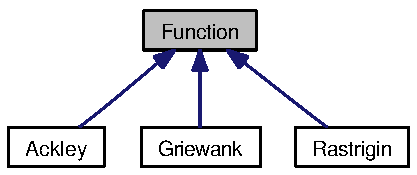
\includegraphics[width=118pt]{classFunction__inherit__graph}
\end{center}
\end{figure}
\subsection*{Public Member Functions}
\begin{CompactItemize}
\item 
virtual double \hyperlink{classFunction_9323a7309b16e0e168590e34b359ff32}{evaluate} (vector$<$ double $>$ \&x)=0
\end{CompactItemize}
\subsection*{Public Attributes}
\begin{CompactItemize}
\item 
int \hyperlink{classFunction_2f582d2da9cb2af5507a55e17bc44083}{n}
\item 
vector$<$ pair$<$ double, double $>$ $>$ \hyperlink{classFunction_e846ed04f4211984a2162b620ee91c81}{constraint}
\end{CompactItemize}


\subsection{Member Function Documentation}
\hypertarget{classFunction_9323a7309b16e0e168590e34b359ff32}{
\index{Function@{Function}!evaluate@{evaluate}}
\index{evaluate@{evaluate}!Function@{Function}}
\subsubsection{\setlength{\rightskip}{0pt plus 5cm}virtual double Function::evaluate (vector$<$ double $>$ \& {\em x})\hspace{0.3cm}{\tt  \mbox{[}pure virtual\mbox{]}}}}
\label{classFunction_9323a7309b16e0e168590e34b359ff32}




Implemented in \hyperlink{classGriewank_c34b1c32bfb7b867c6772db5cc6a727f}{Griewank}, \hyperlink{classAckley_6423fcd54b72322f08357879bac580b6}{Ackley}, and \hyperlink{classRastrigin_aba8c37ab1546da6e7ed47123d179673}{Rastrigin}.

\subsection{Member Data Documentation}
\hypertarget{classFunction_2f582d2da9cb2af5507a55e17bc44083}{
\index{Function@{Function}!n@{n}}
\index{n@{n}!Function@{Function}}
\subsubsection{\setlength{\rightskip}{0pt plus 5cm}int {\bf Function::n}}}
\label{classFunction_2f582d2da9cb2af5507a55e17bc44083}


dimension \hypertarget{classFunction_e846ed04f4211984a2162b620ee91c81}{
\index{Function@{Function}!constraint@{constraint}}
\index{constraint@{constraint}!Function@{Function}}
\subsubsection{\setlength{\rightskip}{0pt plus 5cm}vector$<$pair$<$double, double$>$ $>$ {\bf Function::constraint}}}
\label{classFunction_e846ed04f4211984a2162b620ee91c81}




The documentation for this class was generated from the following file:\begin{CompactItemize}
\item 
\hyperlink{Functions_8h}{Functions.h}\end{CompactItemize}

\hypertarget{classGriewank}{
\section{Griewank Class Reference}
\label{classGriewank}\index{Griewank@{Griewank}}
}
The \hyperlink{classGriewank}{Griewank} function.  


{\tt \#include $<$optfunctions.h$>$}

Inheritance diagram for Griewank:Collaboration diagram for Griewank:\subsection*{Public Member Functions}
\begin{CompactItemize}
\item 
\hyperlink{classGriewank_2a659f93f0b1da7fc9fca34fc371d3af}{Griewank} (int n, \hyperlink{optfunctions_8h_ae9aa3a5dd199a43e77abc2cccf4477e}{dynamicStyle\_\-type} dynamicStyle\_\-in)
\begin{CompactList}\small\item\em Constructor with dimension n. \item\end{CompactList}\item 
\hyperlink{classGriewank_f635212f9d2c41fe20b00c474e461743}{$\sim$Griewank} ()
\begin{CompactList}\small\item\em The allocated ressources are freed. \item\end{CompactList}\item 
double \hyperlink{classGriewank_05917918e68b34e9ed3e794388975f6c}{evaluate} (const vector$<$ double $>$ \&pos)
\begin{CompactList}\small\item\em The evaluation function f(pos). \item\end{CompactList}\end{CompactItemize}


\subsection{Detailed Description}
The \hyperlink{classGriewank}{Griewank} function. 

\subsection{Constructor \& Destructor Documentation}
\hypertarget{classGriewank_2a659f93f0b1da7fc9fca34fc371d3af}{
\index{Griewank@{Griewank}!Griewank@{Griewank}}
\index{Griewank@{Griewank}!Griewank@{Griewank}}
\subsubsection{\setlength{\rightskip}{0pt plus 5cm}Griewank::Griewank (int {\em n}, \/  {\bf dynamicStyle\_\-type} {\em dynamicStyle\_\-in})}}
\label{classGriewank_2a659f93f0b1da7fc9fca34fc371d3af}


Constructor with dimension n. 

\hypertarget{classGriewank_f635212f9d2c41fe20b00c474e461743}{
\index{Griewank@{Griewank}!$\sim$Griewank@{$\sim$Griewank}}
\index{$\sim$Griewank@{$\sim$Griewank}!Griewank@{Griewank}}
\subsubsection{\setlength{\rightskip}{0pt plus 5cm}Griewank::$\sim$Griewank ()}}
\label{classGriewank_f635212f9d2c41fe20b00c474e461743}


The allocated ressources are freed. 



\subsection{Member Function Documentation}
\hypertarget{classGriewank_05917918e68b34e9ed3e794388975f6c}{
\index{Griewank@{Griewank}!evaluate@{evaluate}}
\index{evaluate@{evaluate}!Griewank@{Griewank}}
\subsubsection{\setlength{\rightskip}{0pt plus 5cm}double Griewank::evaluate (const vector$<$ double $>$ \& {\em pos})\hspace{0.3cm}{\tt  \mbox{[}virtual\mbox{]}}}}
\label{classGriewank_05917918e68b34e9ed3e794388975f6c}


The evaluation function f(pos). 



Reimplemented from \hyperlink{classFunction_159260a1fc3afa8932491e4057b6b844}{Function}.

The documentation for this class was generated from the following files:\begin{CompactItemize}
\item 
/home/andrej/workspace/hpso/pso\_\-src/\hyperlink{optfunctions_8h}{optfunctions.h}\item 
/home/andrej/workspace/hpso/pso\_\-src/\hyperlink{optfunctions_8cpp}{optfunctions.cpp}\end{CompactItemize}

\hypertarget{classRandom}{
\section{Random Class Reference}
\label{classRandom}\index{Random@{Random}}
}
{\tt \#include $<$Random.h$>$}

\subsection*{Public Member Functions}
\begin{CompactItemize}
\item 
\hyperlink{classRandom_9a974d20ddfe8d3446b6c5caf1070fab}{Random} (const int \&arg)
\item 
double \hyperlink{classRandom_496fd24cf56a81dc0e0e35bc89e22dd4}{next} ()
\item 
vector$<$ int $>$ \hyperlink{classRandom_d910cd5ff76a472b480f7917fbd7731c}{generate\_\-array} (const int \&size)
\item 
vector$<$ long int $>$ \hyperlink{classRandom_cc60a9ae73a1d6f8bd85211253228d7d}{generate\_\-random\_\-vector} (const int \&size)
\end{CompactItemize}
\subsection*{Public Attributes}
\begin{CompactItemize}
\item 
long int \hyperlink{classRandom_b5bc0589111c5d5198e82cffde01964b}{seed}
\end{CompactItemize}
\subsection*{Private Member Functions}
\begin{CompactItemize}
\item 
double \hyperlink{classRandom_edbbb92c4f516da86f3546021267b7b0}{ran01} (long $\ast$idum)
\end{CompactItemize}
\subsection*{Static Private Attributes}
\begin{CompactItemize}
\item 
static const int \hyperlink{classRandom_d46d9384a3a1d20b9aa4d2476c274993}{IA} = 16807
\item 
static const int \hyperlink{classRandom_951998ee091a5acf5337e1c215e66f6e}{IM} = 2147483647
\item 
static const double \hyperlink{classRandom_12ab86946d6892b1bbca4640314c4836}{AM} = (1.0/\hyperlink{classRandom_951998ee091a5acf5337e1c215e66f6e}{IM})
\item 
static const int \hyperlink{classRandom_7792314b78dc687dfd6a7b511d937c75}{IQ} = 127773
\item 
static const int \hyperlink{classRandom_8c7d5f7cf040525a9111fa69b1d35a38}{IR} = 2836
\end{CompactItemize}


\subsection{Constructor \& Destructor Documentation}
\hypertarget{classRandom_9a974d20ddfe8d3446b6c5caf1070fab}{
\index{Random@{Random}!Random@{Random}}
\index{Random@{Random}!Random@{Random}}
\subsubsection{\setlength{\rightskip}{0pt plus 5cm}Random::Random (const int \& {\em arg})\hspace{0.3cm}{\tt  \mbox{[}inline\mbox{]}}}}
\label{classRandom_9a974d20ddfe8d3446b6c5caf1070fab}




\subsection{Member Function Documentation}
\hypertarget{classRandom_edbbb92c4f516da86f3546021267b7b0}{
\index{Random@{Random}!ran01@{ran01}}
\index{ran01@{ran01}!Random@{Random}}
\subsubsection{\setlength{\rightskip}{0pt plus 5cm}double Random::ran01 (long $\ast$ {\em idum})\hspace{0.3cm}{\tt  \mbox{[}private\mbox{]}}}}
\label{classRandom_edbbb92c4f516da86f3546021267b7b0}


\hypertarget{classRandom_496fd24cf56a81dc0e0e35bc89e22dd4}{
\index{Random@{Random}!next@{next}}
\index{next@{next}!Random@{Random}}
\subsubsection{\setlength{\rightskip}{0pt plus 5cm}double Random::next ()\hspace{0.3cm}{\tt  \mbox{[}inline\mbox{]}}}}
\label{classRandom_496fd24cf56a81dc0e0e35bc89e22dd4}




Here is the call graph for this function:\nopagebreak
\begin{figure}[H]
\begin{center}
\leavevmode
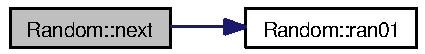
\includegraphics[width=120pt]{classRandom_496fd24cf56a81dc0e0e35bc89e22dd4_cgraph}
\end{center}
\end{figure}
\hypertarget{classRandom_d910cd5ff76a472b480f7917fbd7731c}{
\index{Random@{Random}!generate\_\-array@{generate\_\-array}}
\index{generate\_\-array@{generate\_\-array}!Random@{Random}}
\subsubsection{\setlength{\rightskip}{0pt plus 5cm}vector$<$ int $>$ Random::generate\_\-array (const int \& {\em size})}}
\label{classRandom_d910cd5ff76a472b480f7917fbd7731c}




Here is the call graph for this function:\nopagebreak
\begin{figure}[H]
\begin{center}
\leavevmode
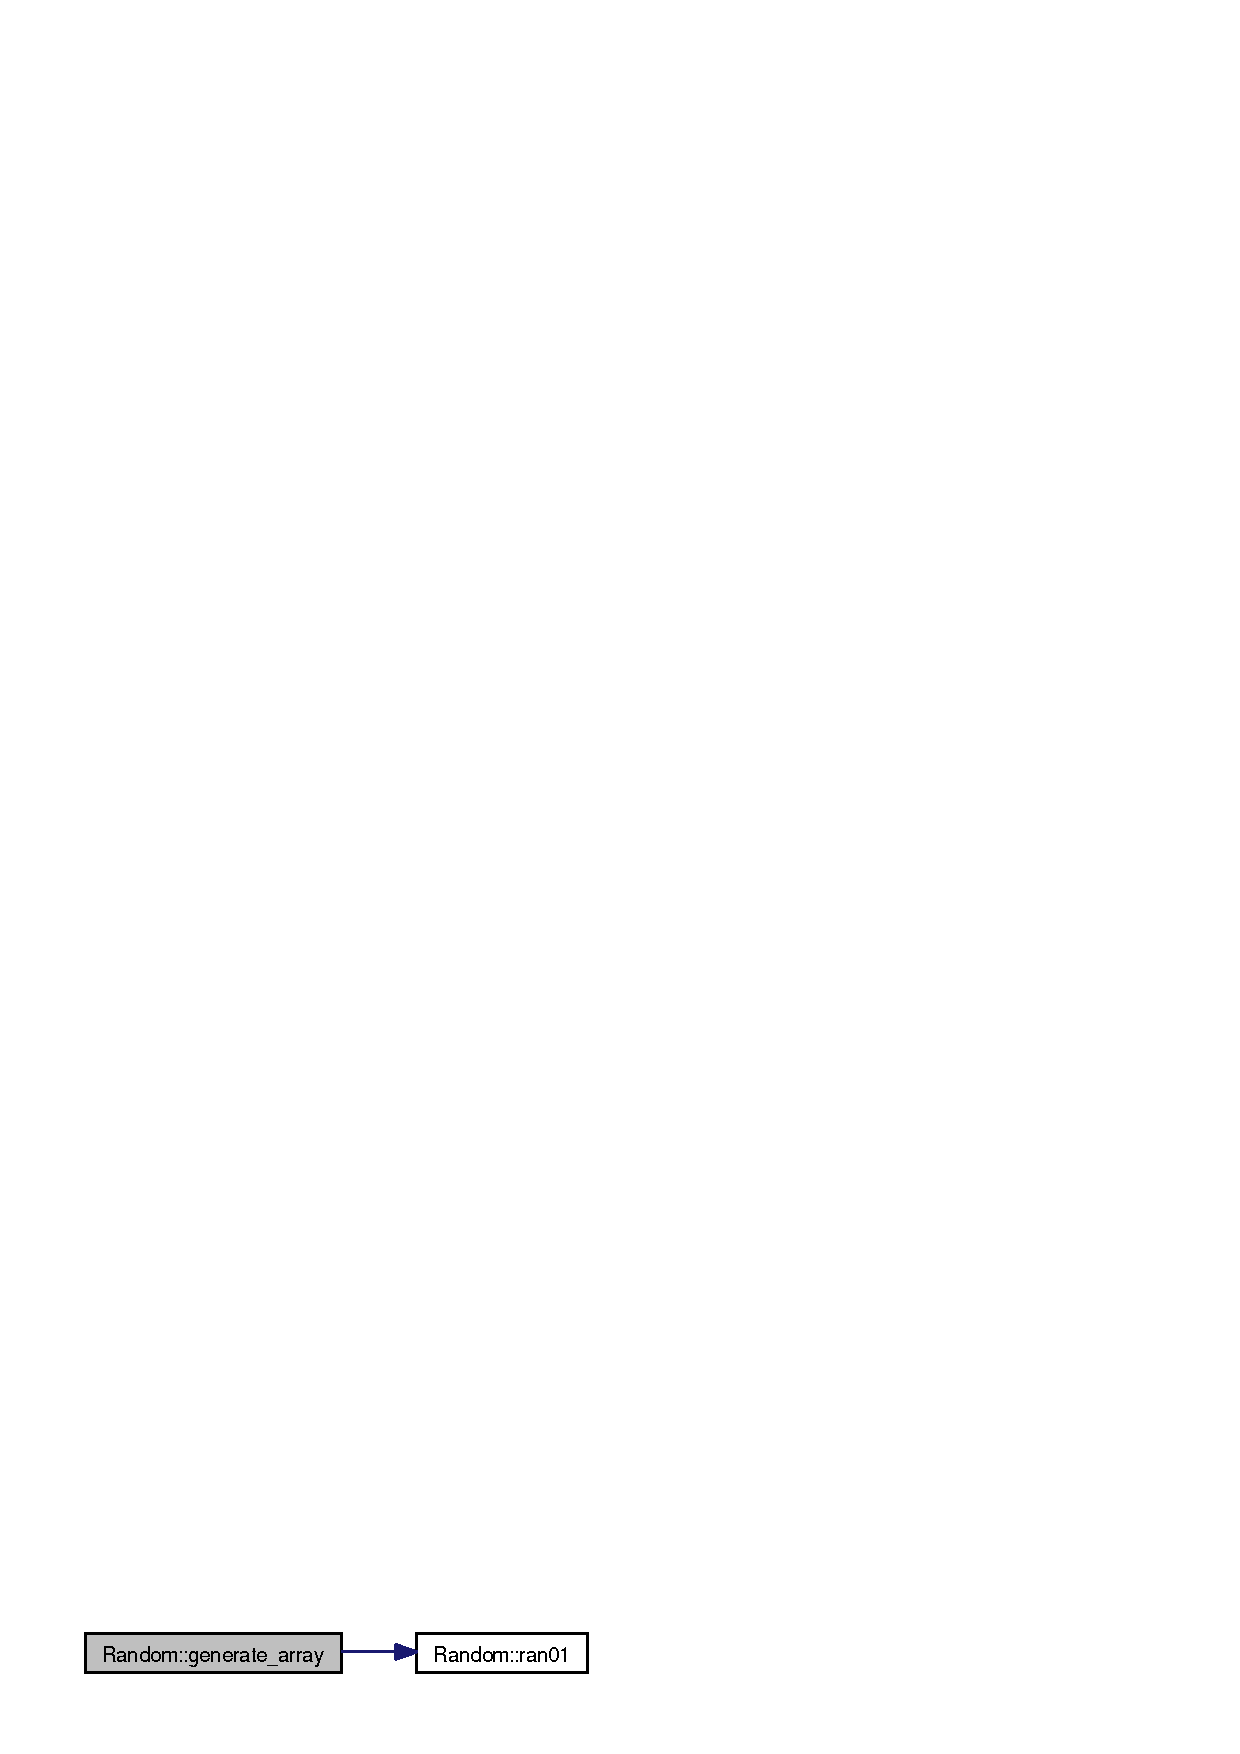
\includegraphics[width=143pt]{classRandom_d910cd5ff76a472b480f7917fbd7731c_cgraph}
\end{center}
\end{figure}
\hypertarget{classRandom_cc60a9ae73a1d6f8bd85211253228d7d}{
\index{Random@{Random}!generate\_\-random\_\-vector@{generate\_\-random\_\-vector}}
\index{generate\_\-random\_\-vector@{generate\_\-random\_\-vector}!Random@{Random}}
\subsubsection{\setlength{\rightskip}{0pt plus 5cm}vector$<$long int$>$ Random::generate\_\-random\_\-vector (const int \& {\em size})\hspace{0.3cm}{\tt  \mbox{[}inline\mbox{]}}}}
\label{classRandom_cc60a9ae73a1d6f8bd85211253228d7d}




\subsection{Member Data Documentation}
\hypertarget{classRandom_d46d9384a3a1d20b9aa4d2476c274993}{
\index{Random@{Random}!IA@{IA}}
\index{IA@{IA}!Random@{Random}}
\subsubsection{\setlength{\rightskip}{0pt plus 5cm}const int {\bf Random::IA} = 16807\hspace{0.3cm}{\tt  \mbox{[}static, private\mbox{]}}}}
\label{classRandom_d46d9384a3a1d20b9aa4d2476c274993}


\hypertarget{classRandom_951998ee091a5acf5337e1c215e66f6e}{
\index{Random@{Random}!IM@{IM}}
\index{IM@{IM}!Random@{Random}}
\subsubsection{\setlength{\rightskip}{0pt plus 5cm}const int {\bf Random::IM} = 2147483647\hspace{0.3cm}{\tt  \mbox{[}static, private\mbox{]}}}}
\label{classRandom_951998ee091a5acf5337e1c215e66f6e}


\hypertarget{classRandom_12ab86946d6892b1bbca4640314c4836}{
\index{Random@{Random}!AM@{AM}}
\index{AM@{AM}!Random@{Random}}
\subsubsection{\setlength{\rightskip}{0pt plus 5cm}const double {\bf Random::AM} = (1.0/{\bf IM})\hspace{0.3cm}{\tt  \mbox{[}static, private\mbox{]}}}}
\label{classRandom_12ab86946d6892b1bbca4640314c4836}


\hypertarget{classRandom_7792314b78dc687dfd6a7b511d937c75}{
\index{Random@{Random}!IQ@{IQ}}
\index{IQ@{IQ}!Random@{Random}}
\subsubsection{\setlength{\rightskip}{0pt plus 5cm}const int {\bf Random::IQ} = 127773\hspace{0.3cm}{\tt  \mbox{[}static, private\mbox{]}}}}
\label{classRandom_7792314b78dc687dfd6a7b511d937c75}


\hypertarget{classRandom_8c7d5f7cf040525a9111fa69b1d35a38}{
\index{Random@{Random}!IR@{IR}}
\index{IR@{IR}!Random@{Random}}
\subsubsection{\setlength{\rightskip}{0pt plus 5cm}const int {\bf Random::IR} = 2836\hspace{0.3cm}{\tt  \mbox{[}static, private\mbox{]}}}}
\label{classRandom_8c7d5f7cf040525a9111fa69b1d35a38}


\hypertarget{classRandom_b5bc0589111c5d5198e82cffde01964b}{
\index{Random@{Random}!seed@{seed}}
\index{seed@{seed}!Random@{Random}}
\subsubsection{\setlength{\rightskip}{0pt plus 5cm}long int {\bf Random::seed}}}
\label{classRandom_b5bc0589111c5d5198e82cffde01964b}




The documentation for this class was generated from the following files:\begin{CompactItemize}
\item 
\hyperlink{Random_8h}{Random.h}\item 
\hyperlink{Random_8cc}{Random.cc}\end{CompactItemize}

\hypertarget{classRastrigin}{
\section{Rastrigin Class Reference}
\label{classRastrigin}\index{Rastrigin@{Rastrigin}}
}
The \hyperlink{classRastrigin}{Rastrigin} function.  


{\tt \#include $<$optfunctions.h$>$}

Inheritance diagram for Rastrigin:Collaboration diagram for Rastrigin:\subsection*{Public Member Functions}
\begin{CompactItemize}
\item 
\hyperlink{classRastrigin_49b26cc4c0afa49a791b35bc2385b17c}{Rastrigin} (int n, \hyperlink{optfunctions_8h_ae9aa3a5dd199a43e77abc2cccf4477e}{dynamicStyle\_\-type} dynamicStyle\_\-in)
\begin{CompactList}\small\item\em Constructor with dimension n. \item\end{CompactList}\item 
\hyperlink{classRastrigin_2d87813baa436f94a5081994faf60662}{$\sim$Rastrigin} ()
\begin{CompactList}\small\item\em The allocated ressources are freed. \item\end{CompactList}\item 
double \hyperlink{classRastrigin_2b969cef4e9fe1a82e6550ab2cb74bd1}{evaluate} (const vector$<$ double $>$ \&pos)
\begin{CompactList}\small\item\em The evaluation function f(pos). \item\end{CompactList}\end{CompactItemize}


\subsection{Detailed Description}
The \hyperlink{classRastrigin}{Rastrigin} function. 

\subsection{Constructor \& Destructor Documentation}
\hypertarget{classRastrigin_49b26cc4c0afa49a791b35bc2385b17c}{
\index{Rastrigin@{Rastrigin}!Rastrigin@{Rastrigin}}
\index{Rastrigin@{Rastrigin}!Rastrigin@{Rastrigin}}
\subsubsection{\setlength{\rightskip}{0pt plus 5cm}Rastrigin::Rastrigin (int {\em n}, \/  {\bf dynamicStyle\_\-type} {\em dynamicStyle\_\-in})}}
\label{classRastrigin_49b26cc4c0afa49a791b35bc2385b17c}


Constructor with dimension n. 

\hypertarget{classRastrigin_2d87813baa436f94a5081994faf60662}{
\index{Rastrigin@{Rastrigin}!$\sim$Rastrigin@{$\sim$Rastrigin}}
\index{$\sim$Rastrigin@{$\sim$Rastrigin}!Rastrigin@{Rastrigin}}
\subsubsection{\setlength{\rightskip}{0pt plus 5cm}Rastrigin::$\sim$Rastrigin ()}}
\label{classRastrigin_2d87813baa436f94a5081994faf60662}


The allocated ressources are freed. 



\subsection{Member Function Documentation}
\hypertarget{classRastrigin_2b969cef4e9fe1a82e6550ab2cb74bd1}{
\index{Rastrigin@{Rastrigin}!evaluate@{evaluate}}
\index{evaluate@{evaluate}!Rastrigin@{Rastrigin}}
\subsubsection{\setlength{\rightskip}{0pt plus 5cm}double Rastrigin::evaluate (const vector$<$ double $>$ \& {\em pos})\hspace{0.3cm}{\tt  \mbox{[}virtual\mbox{]}}}}
\label{classRastrigin_2b969cef4e9fe1a82e6550ab2cb74bd1}


The evaluation function f(pos). 



Reimplemented from \hyperlink{classFunction_159260a1fc3afa8932491e4057b6b844}{Function}.

The documentation for this class was generated from the following files:\begin{CompactItemize}
\item 
/home/andrej/workspace/hpso/pso\_\-src/\hyperlink{optfunctions_8h}{optfunctions.h}\item 
/home/andrej/workspace/hpso/pso\_\-src/\hyperlink{optfunctions_8cpp}{optfunctions.cpp}\end{CompactItemize}

\hypertarget{classSolution}{
\section{Solution Class Reference}
\label{classSolution}\index{Solution@{Solution}}
}
{\tt \#include $<$Solution.h$>$}

\subsection*{Public Attributes}
\begin{CompactItemize}
\item 
vector$<$ double $>$ \hyperlink{classSolution_4b0c127456c4183455b69af7955f15e3}{x}
\item 
double \hyperlink{classSolution_eea6940a1bef4671228f935574883dbc}{value}
\end{CompactItemize}


\subsection{Member Data Documentation}
\hypertarget{classSolution_4b0c127456c4183455b69af7955f15e3}{
\index{Solution@{Solution}!x@{x}}
\index{x@{x}!Solution@{Solution}}
\subsubsection{\setlength{\rightskip}{0pt plus 5cm}vector$<$double$>$ {\bf Solution::x}}}
\label{classSolution_4b0c127456c4183455b69af7955f15e3}


\hypertarget{classSolution_eea6940a1bef4671228f935574883dbc}{
\index{Solution@{Solution}!value@{value}}
\index{value@{value}!Solution@{Solution}}
\subsubsection{\setlength{\rightskip}{0pt plus 5cm}double {\bf Solution::value}}}
\label{classSolution_eea6940a1bef4671228f935574883dbc}




The documentation for this class was generated from the following file:\begin{CompactItemize}
\item 
\hyperlink{Solution_8h}{Solution.h}\end{CompactItemize}

\hypertarget{classTimer}{
\section{Timer Class Reference}
\label{classTimer}\index{Timer@{Timer}}
}
{\tt \#include $<$Timer.h$>$}

\subsection*{Public Types}
\begin{CompactItemize}
\item 
enum \hyperlink{classTimer_f837f758756cde5bdb25c73253e3dd54}{TYPE} \{ \hyperlink{classTimer_f837f758756cde5bdb25c73253e3dd546040915dadd8d1a608e7472b47ebbc91}{REAL}, 
\hyperlink{classTimer_f837f758756cde5bdb25c73253e3dd54e8780921637fe85eab01dda52d0fe2bc}{VIRTUAL}
 \}
\end{CompactItemize}
\subsection*{Public Member Functions}
\begin{CompactItemize}
\item 
\hyperlink{classTimer_f866f8d58d5ed1da7a0c61df4975be3e}{Timer} (void)
\item 
double \hyperlink{classTimer_6ae79acba6fa12eb3c47ad135d4f5a03}{elapsed\_\-time} (const \hyperlink{classTimer_f837f758756cde5bdb25c73253e3dd54}{TYPE} \&type)
\end{CompactItemize}
\subsection*{Private Attributes}
\begin{CompactItemize}
\item 
struct rusage \hyperlink{classTimer_76c056e0461978783ca9c47af3d953d1}{res}
\item 
struct timeval \hyperlink{classTimer_f9d8a85efc3809ca6223ad60bbda6e5a}{tp}
\item 
double \hyperlink{classTimer_1c89ce2e92a2f63cc2309ed9ac765905}{virtual\_\-time}
\item 
double \hyperlink{classTimer_845cc39afdf6c74225d2d5580de49208}{real\_\-time}
\end{CompactItemize}


\subsection{Member Enumeration Documentation}
\hypertarget{classTimer_f837f758756cde5bdb25c73253e3dd54}{
\index{Timer@{Timer}!TYPE@{TYPE}}
\index{TYPE@{TYPE}!Timer@{Timer}}
\subsubsection{\setlength{\rightskip}{0pt plus 5cm}enum {\bf Timer::TYPE}}}
\label{classTimer_f837f758756cde5bdb25c73253e3dd54}


\begin{Desc}
\item[Enumerator: ]\par
\begin{description}
\index{REAL@{REAL}!Timer@{Timer}}\index{Timer@{Timer}!REAL@{REAL}}\item[{\em 
\hypertarget{classTimer_f837f758756cde5bdb25c73253e3dd546040915dadd8d1a608e7472b47ebbc91}{
REAL}
\label{classTimer_f837f758756cde5bdb25c73253e3dd546040915dadd8d1a608e7472b47ebbc91}
}]\index{VIRTUAL@{VIRTUAL}!Timer@{Timer}}\index{Timer@{Timer}!VIRTUAL@{VIRTUAL}}\item[{\em 
\hypertarget{classTimer_f837f758756cde5bdb25c73253e3dd54e8780921637fe85eab01dda52d0fe2bc}{
VIRTUAL}
\label{classTimer_f837f758756cde5bdb25c73253e3dd54e8780921637fe85eab01dda52d0fe2bc}
}]\end{description}
\end{Desc}



\subsection{Constructor \& Destructor Documentation}
\hypertarget{classTimer_f866f8d58d5ed1da7a0c61df4975be3e}{
\index{Timer@{Timer}!Timer@{Timer}}
\index{Timer@{Timer}!Timer@{Timer}}
\subsubsection{\setlength{\rightskip}{0pt plus 5cm}Timer::Timer (void)}}
\label{classTimer_f866f8d58d5ed1da7a0c61df4975be3e}




\subsection{Member Function Documentation}
\hypertarget{classTimer_6ae79acba6fa12eb3c47ad135d4f5a03}{
\index{Timer@{Timer}!elapsed\_\-time@{elapsed\_\-time}}
\index{elapsed\_\-time@{elapsed\_\-time}!Timer@{Timer}}
\subsubsection{\setlength{\rightskip}{0pt plus 5cm}double Timer::elapsed\_\-time (const {\bf TYPE} \& {\em type})}}
\label{classTimer_6ae79acba6fa12eb3c47ad135d4f5a03}




\subsection{Member Data Documentation}
\hypertarget{classTimer_76c056e0461978783ca9c47af3d953d1}{
\index{Timer@{Timer}!res@{res}}
\index{res@{res}!Timer@{Timer}}
\subsubsection{\setlength{\rightskip}{0pt plus 5cm}struct rusage {\bf Timer::res}\hspace{0.3cm}{\tt  \mbox{[}read, private\mbox{]}}}}
\label{classTimer_76c056e0461978783ca9c47af3d953d1}


\hypertarget{classTimer_f9d8a85efc3809ca6223ad60bbda6e5a}{
\index{Timer@{Timer}!tp@{tp}}
\index{tp@{tp}!Timer@{Timer}}
\subsubsection{\setlength{\rightskip}{0pt plus 5cm}struct timeval {\bf Timer::tp}\hspace{0.3cm}{\tt  \mbox{[}read, private\mbox{]}}}}
\label{classTimer_f9d8a85efc3809ca6223ad60bbda6e5a}


\hypertarget{classTimer_1c89ce2e92a2f63cc2309ed9ac765905}{
\index{Timer@{Timer}!virtual\_\-time@{virtual\_\-time}}
\index{virtual\_\-time@{virtual\_\-time}!Timer@{Timer}}
\subsubsection{\setlength{\rightskip}{0pt plus 5cm}double {\bf Timer::virtual\_\-time}\hspace{0.3cm}{\tt  \mbox{[}private\mbox{]}}}}
\label{classTimer_1c89ce2e92a2f63cc2309ed9ac765905}


\hypertarget{classTimer_845cc39afdf6c74225d2d5580de49208}{
\index{Timer@{Timer}!real\_\-time@{real\_\-time}}
\index{real\_\-time@{real\_\-time}!Timer@{Timer}}
\subsubsection{\setlength{\rightskip}{0pt plus 5cm}double {\bf Timer::real\_\-time}\hspace{0.3cm}{\tt  \mbox{[}private\mbox{]}}}}
\label{classTimer_845cc39afdf6c74225d2d5580de49208}




The documentation for this class was generated from the following files:\begin{CompactItemize}
\item 
\hyperlink{Timer_8h}{Timer.h}\item 
\hyperlink{Timer_8cc}{Timer.cc}\end{CompactItemize}

\chapter{File Documentation}
\hypertarget{aco-r_8cpp}{
\section{aco-r.cpp File Reference}
\label{aco-r_8cpp}\index{aco-r.cpp@{aco-r.cpp}}
}
{\tt \#include \char`\"{}Timer.h\char`\"{}}\par
{\tt \#include \char`\"{}Solution.h\char`\"{}}\par
{\tt \#include \char`\"{}Functions.h\char`\"{}}\par
{\tt \#include $<$string$>$}\par
{\tt \#include $<$list$>$}\par
{\tt \#include $<$map$>$}\par
{\tt \#include $<$stdio.h$>$}\par
{\tt \#include $<$stdlib.h$>$}\par
{\tt \#include $<$iostream$>$}\par
{\tt \#include $<$math.h$>$}\par
{\tt \#include $<$ctime$>$}\par
{\tt \#include $<$cstdlib$>$}\par


Include dependency graph for aco-r.cpp:\nopagebreak
\begin{figure}[H]
\begin{center}
\leavevmode
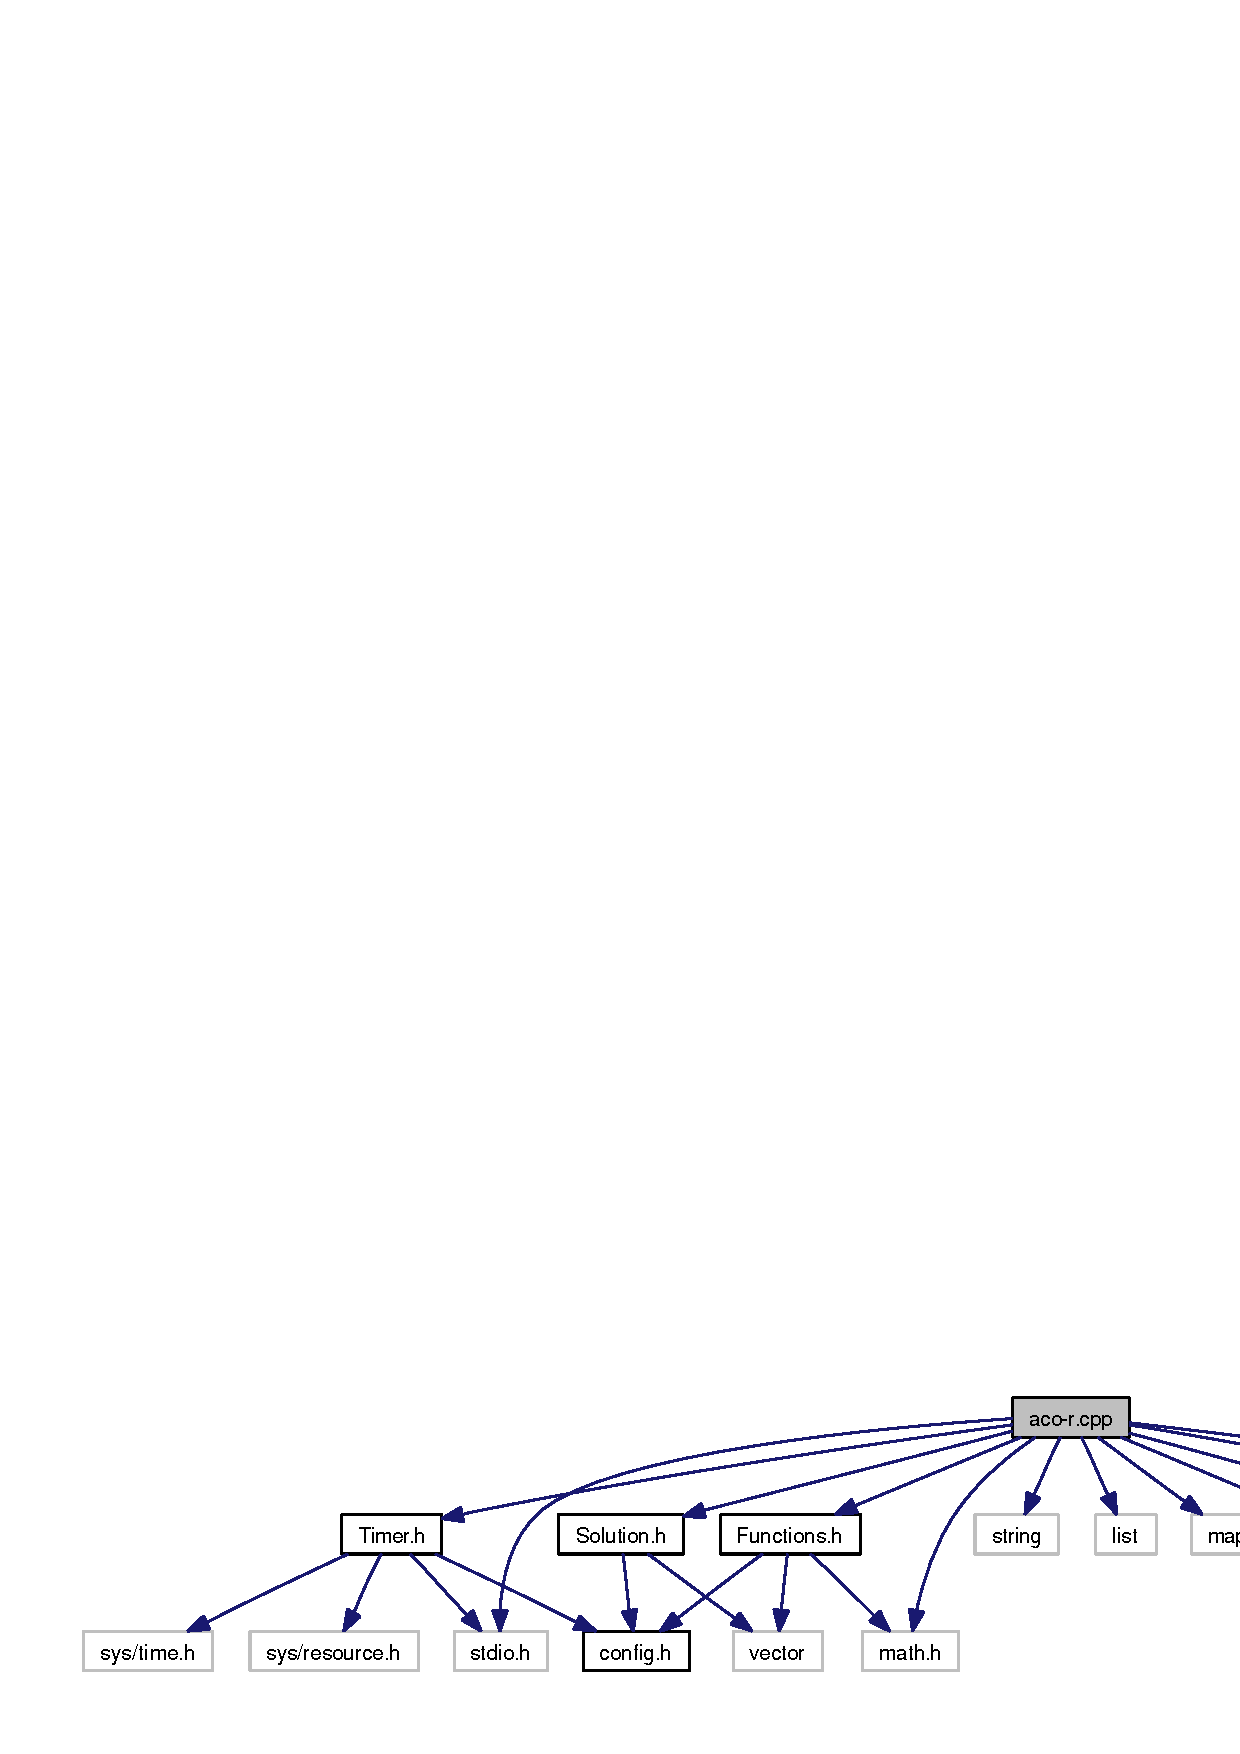
\includegraphics[width=420pt]{aco-r_8cpp__incl}
\end{center}
\end{figure}
\subsection*{Defines}
\begin{CompactItemize}
\item 
\#define \hyperlink{aco-r_8cpp_523b1c70fbff9e4e25f29b323bead209}{RAND\_\-UNIFORME}~(double)random()/(double)RAND\_\-MAX
\end{CompactItemize}
\subsection*{Functions}
\begin{CompactItemize}
\item 
void \hyperlink{aco-r_8cpp_02fd73d861ef2e4aabb38c0c9ff82947}{init} ()
\item 
double \hyperlink{aco-r_8cpp_c49c8f28940eb73a2d3c5d4f54a77acb}{gaussian} (double mean, double var)
\item 
void \hyperlink{aco-r_8cpp_cec77708e3d6f73a14c252e8747c11b1}{print\_\-best\_\-solution} (\hyperlink{classSolution}{Solution} bSol, \hyperlink{classFunction}{Function} $\ast$af, \hyperlink{classTimer}{Timer} \&atimer, int icount)
\item 
double \hyperlink{aco-r_8cpp_c5992296530c3f2c91fb35345606b029}{evaluate} (double $\ast$s)
\item 
int \hyperlink{aco-r_8cpp_3c04138a5bfe5d72780bb7e82a18e627}{main} (int argc, char $\ast$$\ast$argv)
\end{CompactItemize}
\subsection*{Variables}
\begin{CompactItemize}
\item 
double $\ast$ \hyperlink{aco-r_8cpp_a0e91b6673e0f6c62ed362a35d18064e}{archive} = NULL
\item 
double $\ast$ \hyperlink{aco-r_8cpp_68e32a83dbc9e45c0eca86384c297aba}{constrains} = NULL
\item 
int \hyperlink{aco-r_8cpp_1a8a8235879363159315091a1daed72f}{dimension} = 10
\item 
int \hyperlink{aco-r_8cpp_ae8c272782ff802dd95092adf15f474e}{archive\_\-size} = 5
\item 
int \hyperlink{aco-r_8cpp_346cfde20df32ef1244e37b7de85f5a3}{number\_\-of\_\-ants} = 3
\item 
int \hyperlink{aco-r_8cpp_77d5d27d8fdf89eb369e3bae9e6e752d}{number\_\-of\_\-iterations} = 100
\item 
double \hyperlink{aco-r_8cpp_5b5e3f03e443adea974601f295136638}{q} = 1.0
\item 
double \hyperlink{aco-r_8cpp_3ed57096651b587c2bf716fa78048153}{rho} = 1.0
\end{CompactItemize}


\subsection{Define Documentation}
\hypertarget{aco-r_8cpp_523b1c70fbff9e4e25f29b323bead209}{
\index{aco-r.cpp@{aco-r.cpp}!RAND\_\-UNIFORME@{RAND\_\-UNIFORME}}
\index{RAND\_\-UNIFORME@{RAND\_\-UNIFORME}!aco-r.cpp@{aco-r.cpp}}
\subsubsection{\setlength{\rightskip}{0pt plus 5cm}\#define RAND\_\-UNIFORME~(double)random()/(double)RAND\_\-MAX}}
\label{aco-r_8cpp_523b1c70fbff9e4e25f29b323bead209}




\subsection{Function Documentation}
\hypertarget{aco-r_8cpp_c5992296530c3f2c91fb35345606b029}{
\index{aco-r.cpp@{aco-r.cpp}!evaluate@{evaluate}}
\index{evaluate@{evaluate}!aco-r.cpp@{aco-r.cpp}}
\subsubsection{\setlength{\rightskip}{0pt plus 5cm}double evaluate (double $\ast$ {\em s})}}
\label{aco-r_8cpp_c5992296530c3f2c91fb35345606b029}


\hypertarget{aco-r_8cpp_c49c8f28940eb73a2d3c5d4f54a77acb}{
\index{aco-r.cpp@{aco-r.cpp}!gaussian@{gaussian}}
\index{gaussian@{gaussian}!aco-r.cpp@{aco-r.cpp}}
\subsubsection{\setlength{\rightskip}{0pt plus 5cm}double gaussian (double {\em mean}, \/  double {\em var})}}
\label{aco-r_8cpp_c49c8f28940eb73a2d3c5d4f54a77acb}


\hypertarget{aco-r_8cpp_02fd73d861ef2e4aabb38c0c9ff82947}{
\index{aco-r.cpp@{aco-r.cpp}!init@{init}}
\index{init@{init}!aco-r.cpp@{aco-r.cpp}}
\subsubsection{\setlength{\rightskip}{0pt plus 5cm}void init ()}}
\label{aco-r_8cpp_02fd73d861ef2e4aabb38c0c9ff82947}


\hypertarget{aco-r_8cpp_3c04138a5bfe5d72780bb7e82a18e627}{
\index{aco-r.cpp@{aco-r.cpp}!main@{main}}
\index{main@{main}!aco-r.cpp@{aco-r.cpp}}
\subsubsection{\setlength{\rightskip}{0pt plus 5cm}int main (int {\em argc}, \/  char $\ast$$\ast$ {\em argv})}}
\label{aco-r_8cpp_3c04138a5bfe5d72780bb7e82a18e627}




Here is the call graph for this function:\nopagebreak
\begin{figure}[H]
\begin{center}
\leavevmode
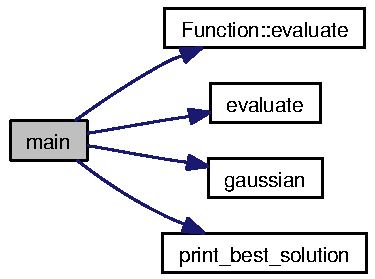
\includegraphics[width=108pt]{aco-r_8cpp_3c04138a5bfe5d72780bb7e82a18e627_cgraph}
\end{center}
\end{figure}
\hypertarget{aco-r_8cpp_cec77708e3d6f73a14c252e8747c11b1}{
\index{aco-r.cpp@{aco-r.cpp}!print\_\-best\_\-solution@{print\_\-best\_\-solution}}
\index{print\_\-best\_\-solution@{print\_\-best\_\-solution}!aco-r.cpp@{aco-r.cpp}}
\subsubsection{\setlength{\rightskip}{0pt plus 5cm}void print\_\-best\_\-solution ({\bf Solution} {\em bSol}, \/  {\bf Function} $\ast$ {\em af}, \/  {\bf Timer} \& {\em atimer}, \/  int {\em icount})}}
\label{aco-r_8cpp_cec77708e3d6f73a14c252e8747c11b1}




\subsection{Variable Documentation}
\hypertarget{aco-r_8cpp_a0e91b6673e0f6c62ed362a35d18064e}{
\index{aco-r.cpp@{aco-r.cpp}!archive@{archive}}
\index{archive@{archive}!aco-r.cpp@{aco-r.cpp}}
\subsubsection{\setlength{\rightskip}{0pt plus 5cm}double$\ast$ {\bf archive} = NULL}}
\label{aco-r_8cpp_a0e91b6673e0f6c62ed362a35d18064e}


\hypertarget{aco-r_8cpp_ae8c272782ff802dd95092adf15f474e}{
\index{aco-r.cpp@{aco-r.cpp}!archive\_\-size@{archive\_\-size}}
\index{archive\_\-size@{archive\_\-size}!aco-r.cpp@{aco-r.cpp}}
\subsubsection{\setlength{\rightskip}{0pt plus 5cm}int {\bf archive\_\-size} = 5}}
\label{aco-r_8cpp_ae8c272782ff802dd95092adf15f474e}


\hypertarget{aco-r_8cpp_68e32a83dbc9e45c0eca86384c297aba}{
\index{aco-r.cpp@{aco-r.cpp}!constrains@{constrains}}
\index{constrains@{constrains}!aco-r.cpp@{aco-r.cpp}}
\subsubsection{\setlength{\rightskip}{0pt plus 5cm}double$\ast$ {\bf constrains} = NULL}}
\label{aco-r_8cpp_68e32a83dbc9e45c0eca86384c297aba}


\hypertarget{aco-r_8cpp_1a8a8235879363159315091a1daed72f}{
\index{aco-r.cpp@{aco-r.cpp}!dimension@{dimension}}
\index{dimension@{dimension}!aco-r.cpp@{aco-r.cpp}}
\subsubsection{\setlength{\rightskip}{0pt plus 5cm}int {\bf dimension} = 10}}
\label{aco-r_8cpp_1a8a8235879363159315091a1daed72f}


\hypertarget{aco-r_8cpp_346cfde20df32ef1244e37b7de85f5a3}{
\index{aco-r.cpp@{aco-r.cpp}!number\_\-of\_\-ants@{number\_\-of\_\-ants}}
\index{number\_\-of\_\-ants@{number\_\-of\_\-ants}!aco-r.cpp@{aco-r.cpp}}
\subsubsection{\setlength{\rightskip}{0pt plus 5cm}int {\bf number\_\-of\_\-ants} = 3}}
\label{aco-r_8cpp_346cfde20df32ef1244e37b7de85f5a3}


\hypertarget{aco-r_8cpp_77d5d27d8fdf89eb369e3bae9e6e752d}{
\index{aco-r.cpp@{aco-r.cpp}!number\_\-of\_\-iterations@{number\_\-of\_\-iterations}}
\index{number\_\-of\_\-iterations@{number\_\-of\_\-iterations}!aco-r.cpp@{aco-r.cpp}}
\subsubsection{\setlength{\rightskip}{0pt plus 5cm}int {\bf number\_\-of\_\-iterations} = 100}}
\label{aco-r_8cpp_77d5d27d8fdf89eb369e3bae9e6e752d}


\hypertarget{aco-r_8cpp_5b5e3f03e443adea974601f295136638}{
\index{aco-r.cpp@{aco-r.cpp}!q@{q}}
\index{q@{q}!aco-r.cpp@{aco-r.cpp}}
\subsubsection{\setlength{\rightskip}{0pt plus 5cm}double {\bf q} = 1.0}}
\label{aco-r_8cpp_5b5e3f03e443adea974601f295136638}


\hypertarget{aco-r_8cpp_3ed57096651b587c2bf716fa78048153}{
\index{aco-r.cpp@{aco-r.cpp}!rho@{rho}}
\index{rho@{rho}!aco-r.cpp@{aco-r.cpp}}
\subsubsection{\setlength{\rightskip}{0pt plus 5cm}double {\bf rho} = 1.0}}
\label{aco-r_8cpp_3ed57096651b587c2bf716fa78048153}



\hypertarget{Colony_8cpp}{
\section{Colony.cpp File Reference}
\label{Colony_8cpp}\index{Colony.cpp@{Colony.cpp}}
}
{\tt \#include $<$iostream$>$}\par
{\tt \#include $<$fstream$>$}\par
{\tt \#include $<$stdio.h$>$}\par
{\tt \#include \char`\"{}Colony.h\char`\"{}}\par


Include dependency graph for Colony.cpp:\nopagebreak
\begin{figure}[H]
\begin{center}
\leavevmode
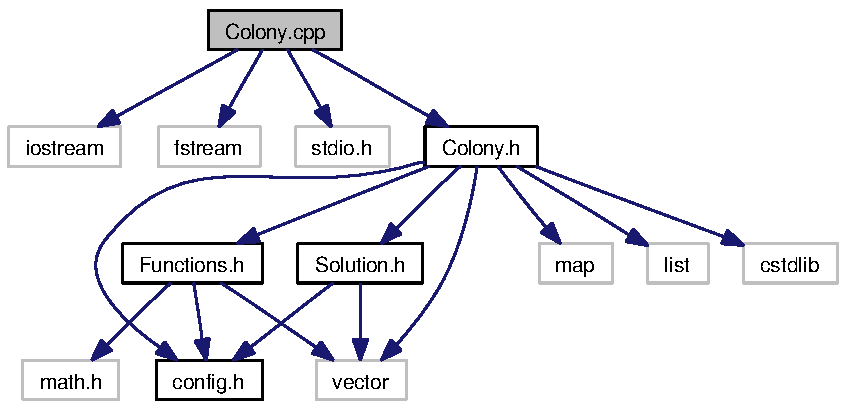
\includegraphics[width=220pt]{Colony_8cpp__incl}
\end{center}
\end{figure}

\hypertarget{Colony_8h}{
\section{Colony.h File Reference}
\label{Colony_8h}\index{Colony.h@{Colony.h}}
}
{\tt \#include \char`\"{}config.h\char`\"{}}\par
{\tt \#include $<$vector$>$}\par
{\tt \#include $<$map$>$}\par
{\tt \#include $<$list$>$}\par
{\tt \#include $<$cstdlib$>$}\par
{\tt \#include \char`\"{}Solution.h\char`\"{}}\par
{\tt \#include \char`\"{}Functions.h\char`\"{}}\par


Include dependency graph for Colony.h:\nopagebreak
\begin{figure}[H]
\begin{center}
\leavevmode
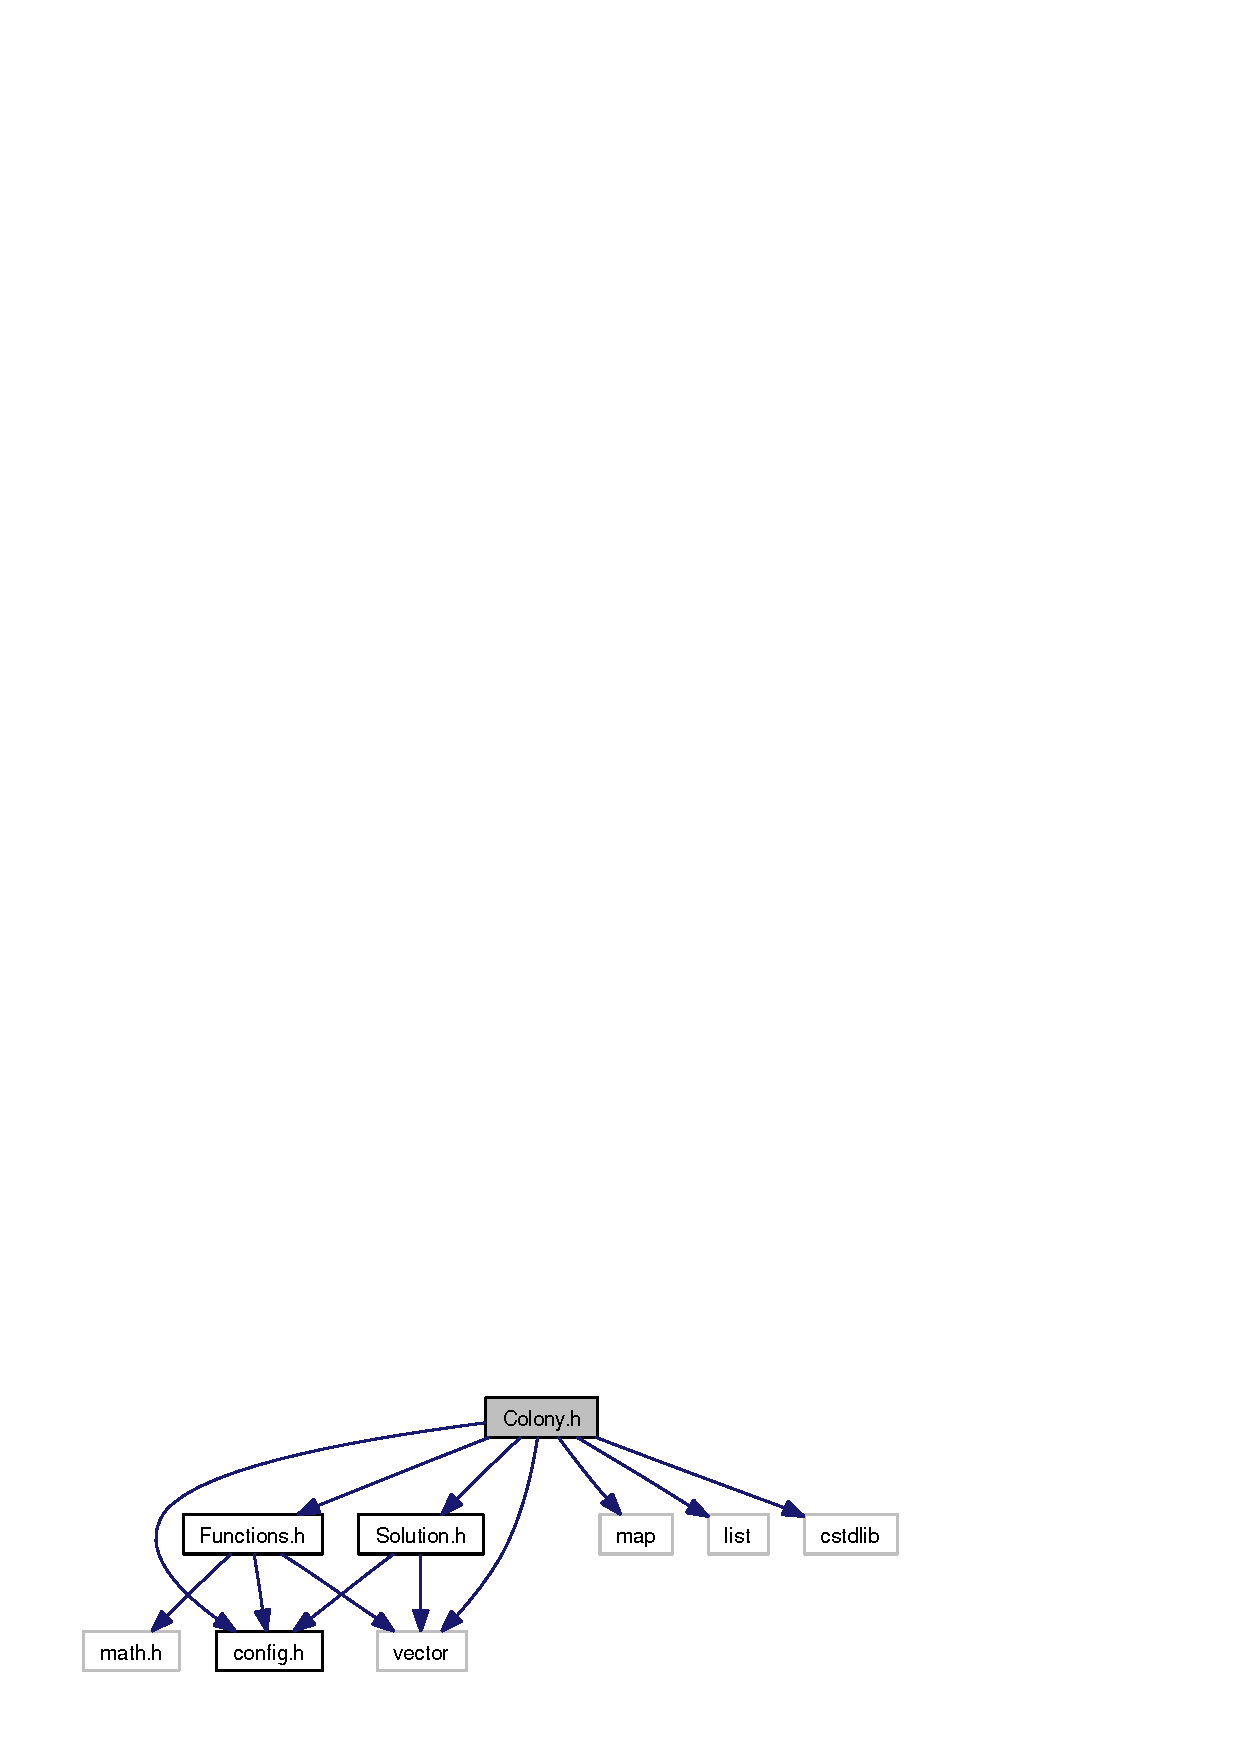
\includegraphics[width=217pt]{Colony_8h__incl}
\end{center}
\end{figure}


This graph shows which files directly or indirectly include this file:\nopagebreak
\begin{figure}[H]
\begin{center}
\leavevmode
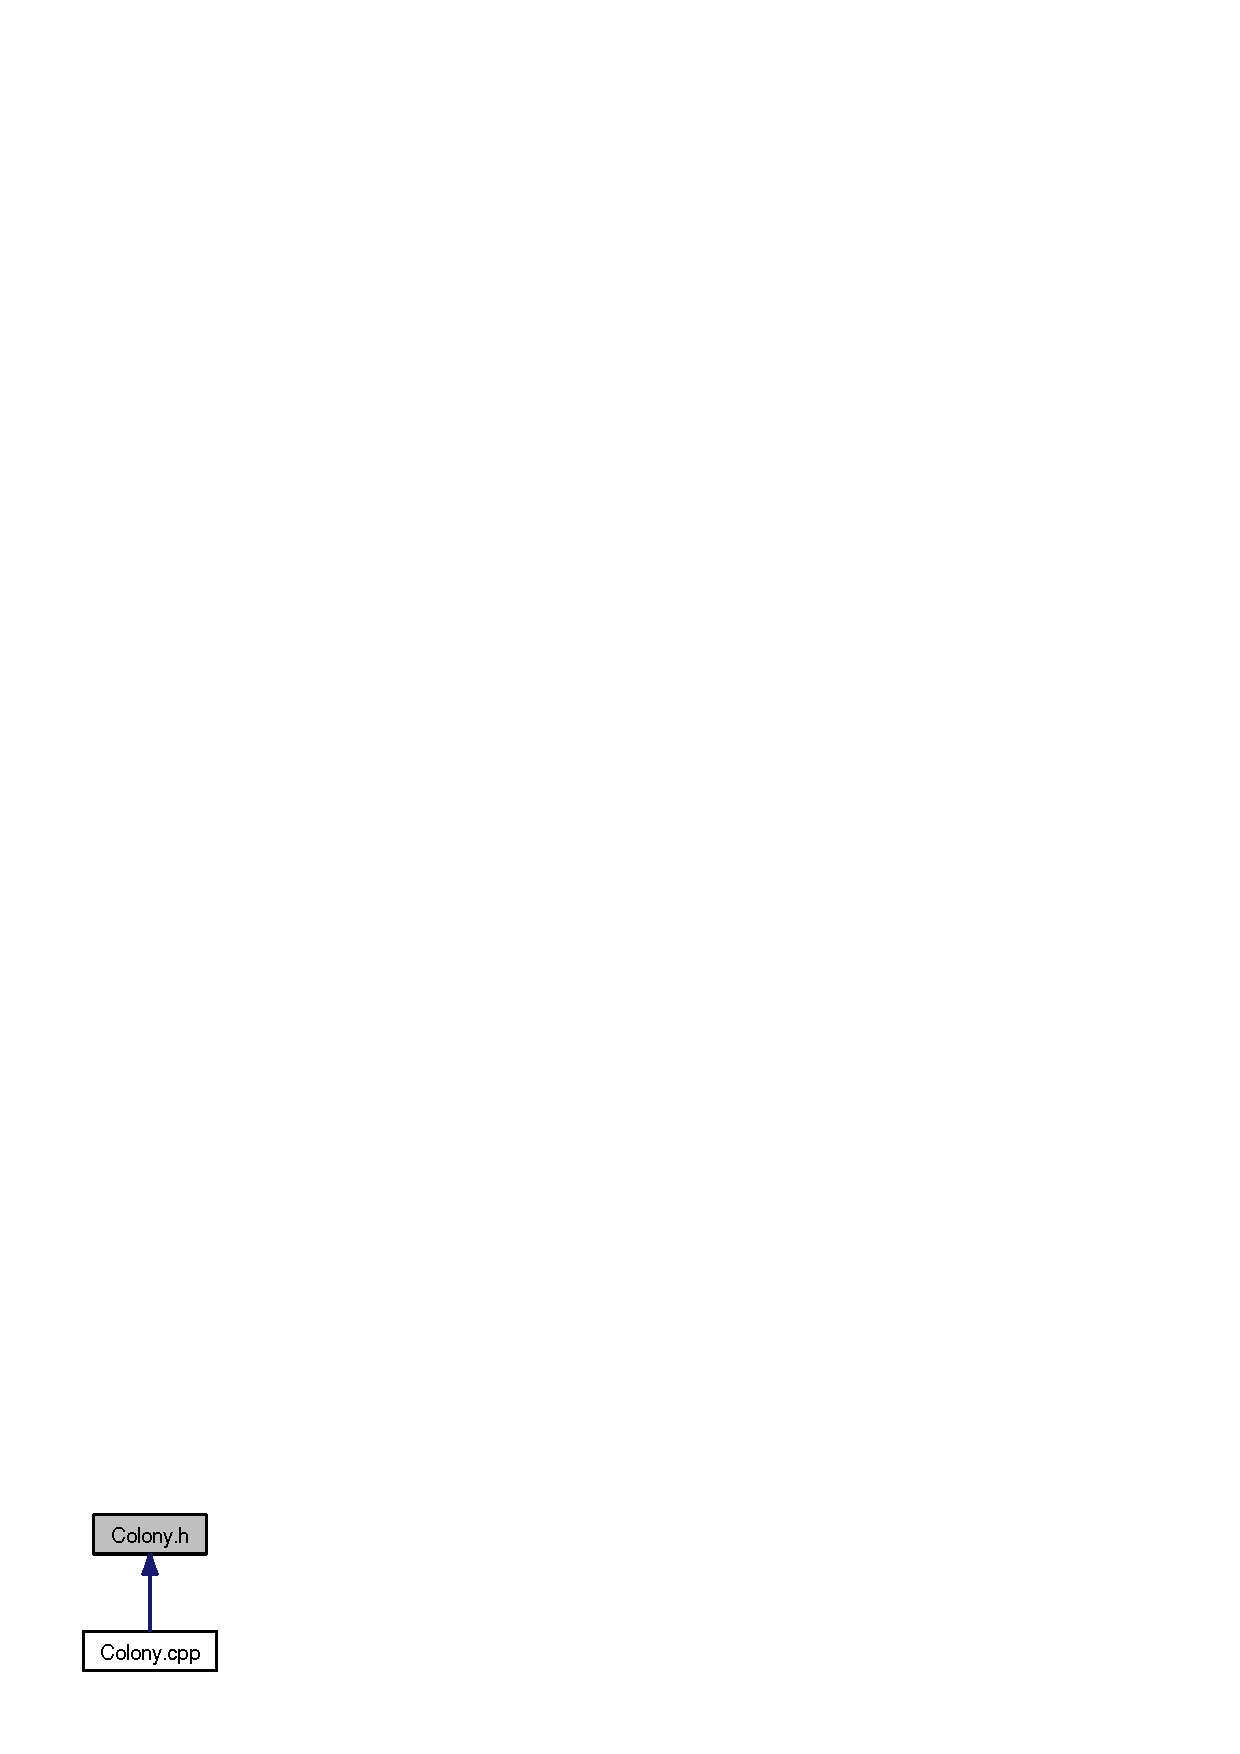
\includegraphics[width=54pt]{Colony_8h__dep__incl}
\end{center}
\end{figure}
\subsection*{Classes}
\begin{CompactItemize}
\item 
class \hyperlink{classColony}{Colony}
\end{CompactItemize}

\hypertarget{config_8h}{
\section{config.h File Reference}
\label{config_8h}\index{config.h@{config.h}}
}


This graph shows which files directly or indirectly include this file:\nopagebreak
\begin{figure}[H]
\begin{center}
\leavevmode
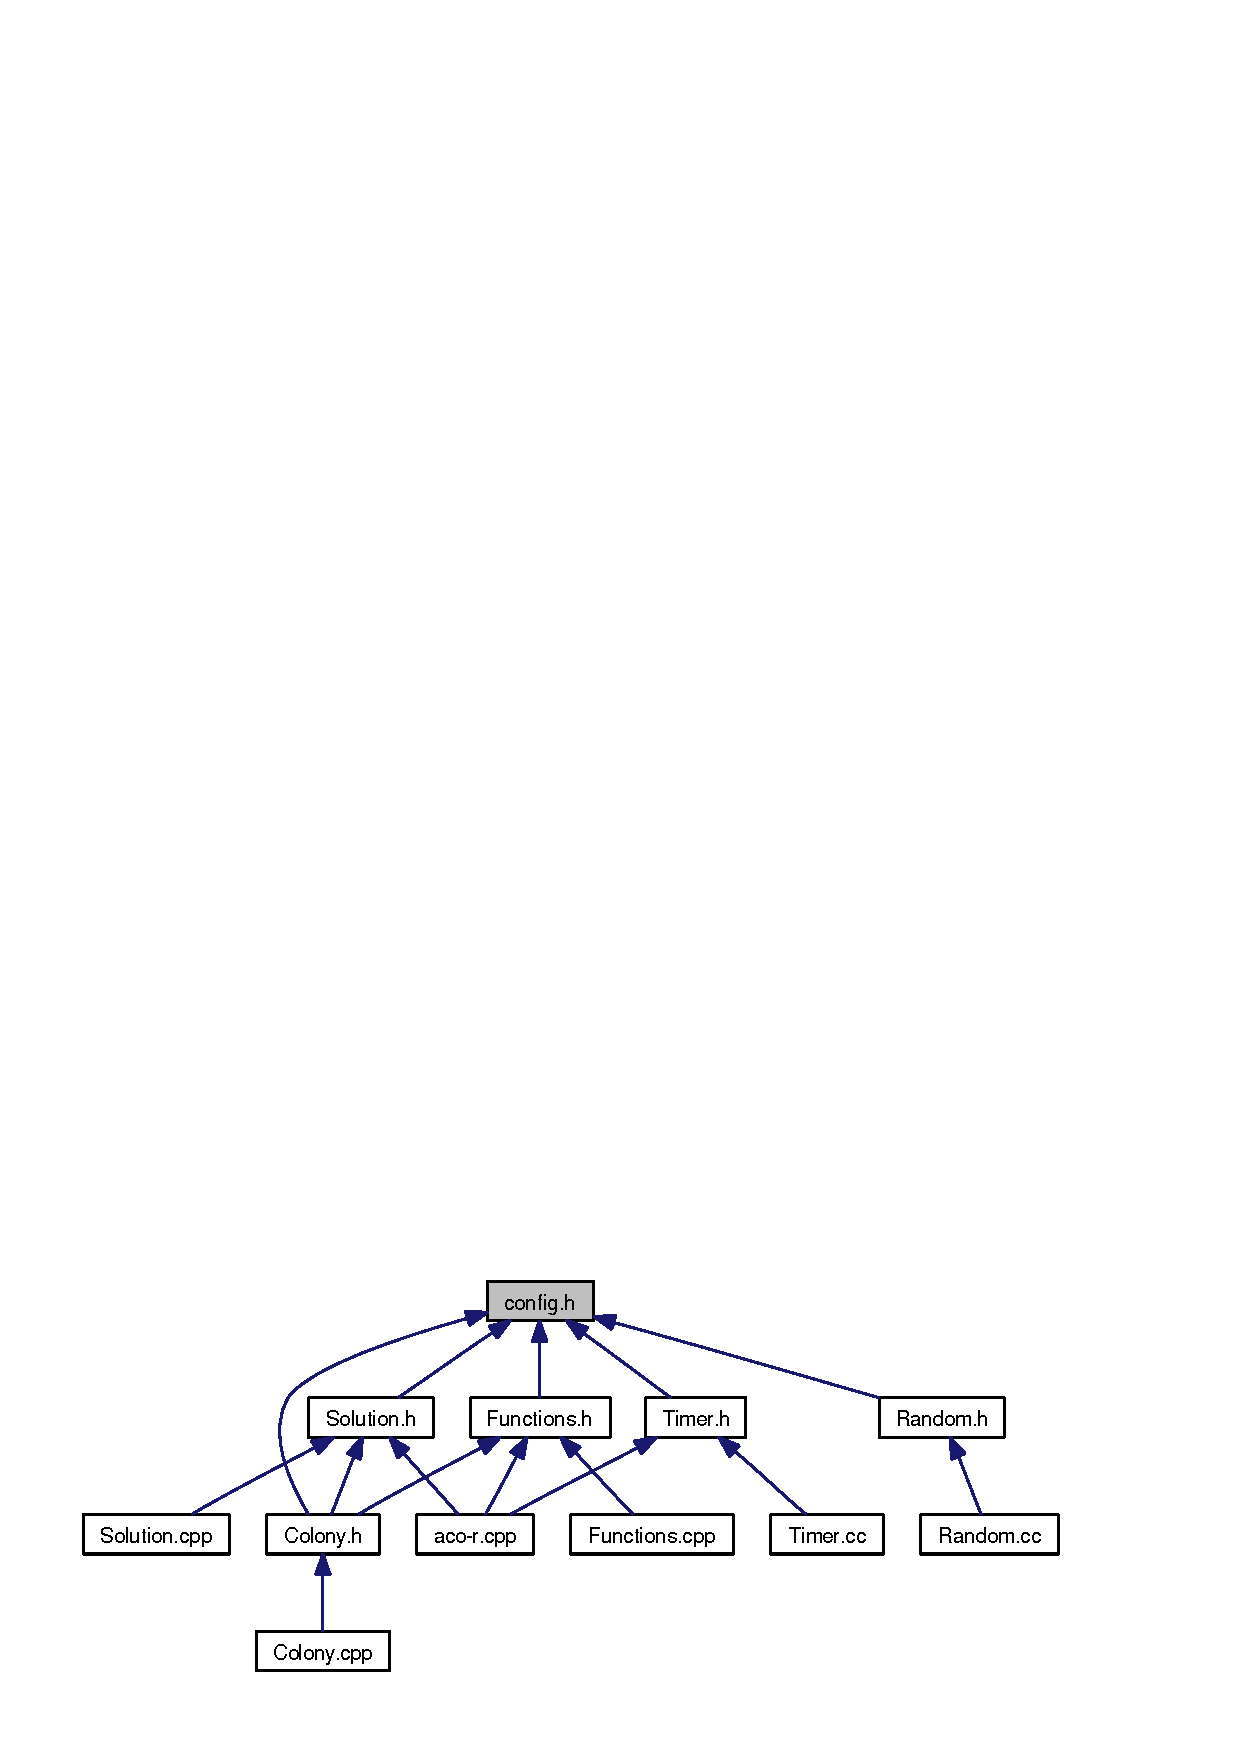
\includegraphics[width=256pt]{config_8h__dep__incl}
\end{center}
\end{figure}

\hypertarget{Functions_8cpp}{
\section{Functions.cpp File Reference}
\label{Functions_8cpp}\index{Functions.cpp@{Functions.cpp}}
}
{\tt \#include \char`\"{}Functions.h\char`\"{}}\par


Include dependency graph for Functions.cpp:\nopagebreak
\begin{figure}[H]
\begin{center}
\leavevmode
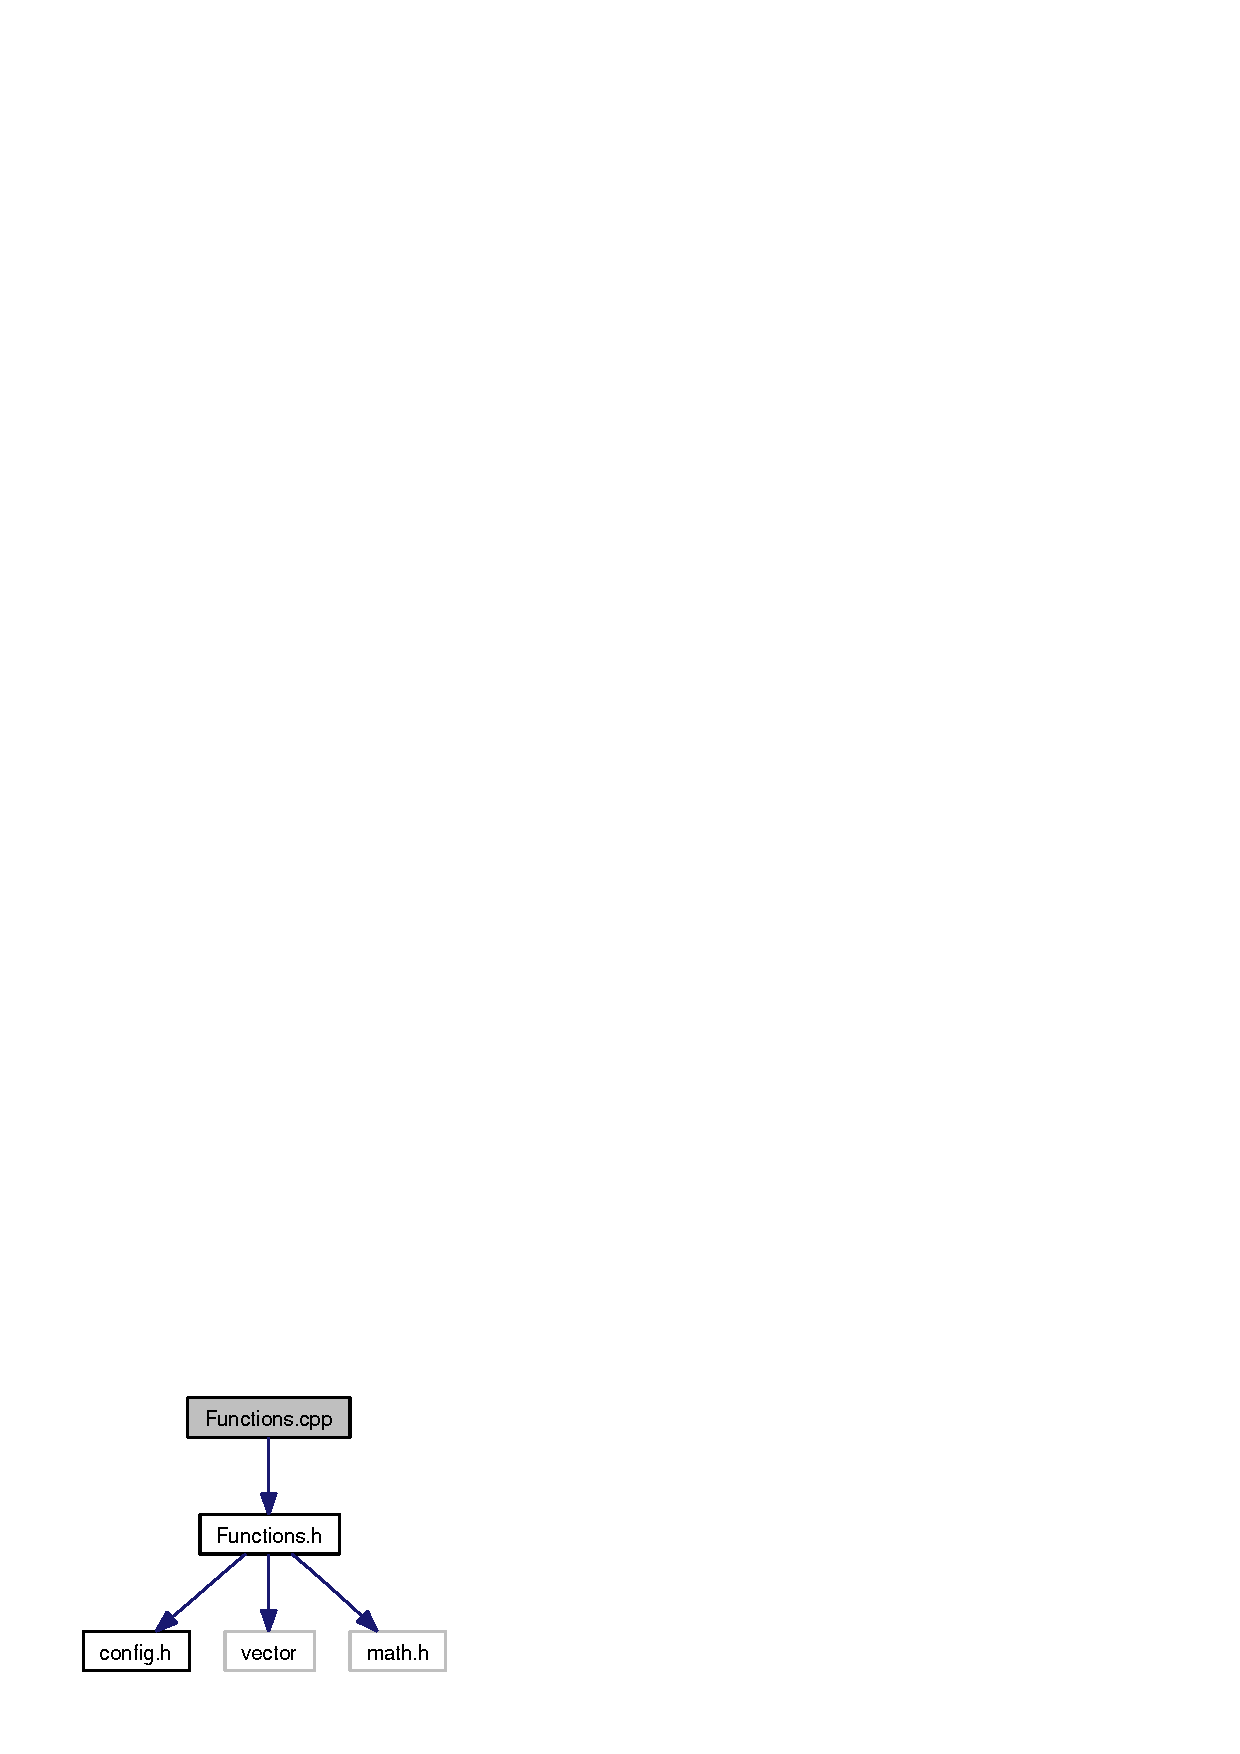
\includegraphics[width=109pt]{Functions_8cpp__incl}
\end{center}
\end{figure}

\hypertarget{Functions_8h}{
\section{Functions.h File Reference}
\label{Functions_8h}\index{Functions.h@{Functions.h}}
}
{\tt \#include \char`\"{}config.h\char`\"{}}\par
{\tt \#include $<$vector$>$}\par
{\tt \#include $<$math.h$>$}\par


Include dependency graph for Functions.h:\nopagebreak
\begin{figure}[H]
\begin{center}
\leavevmode
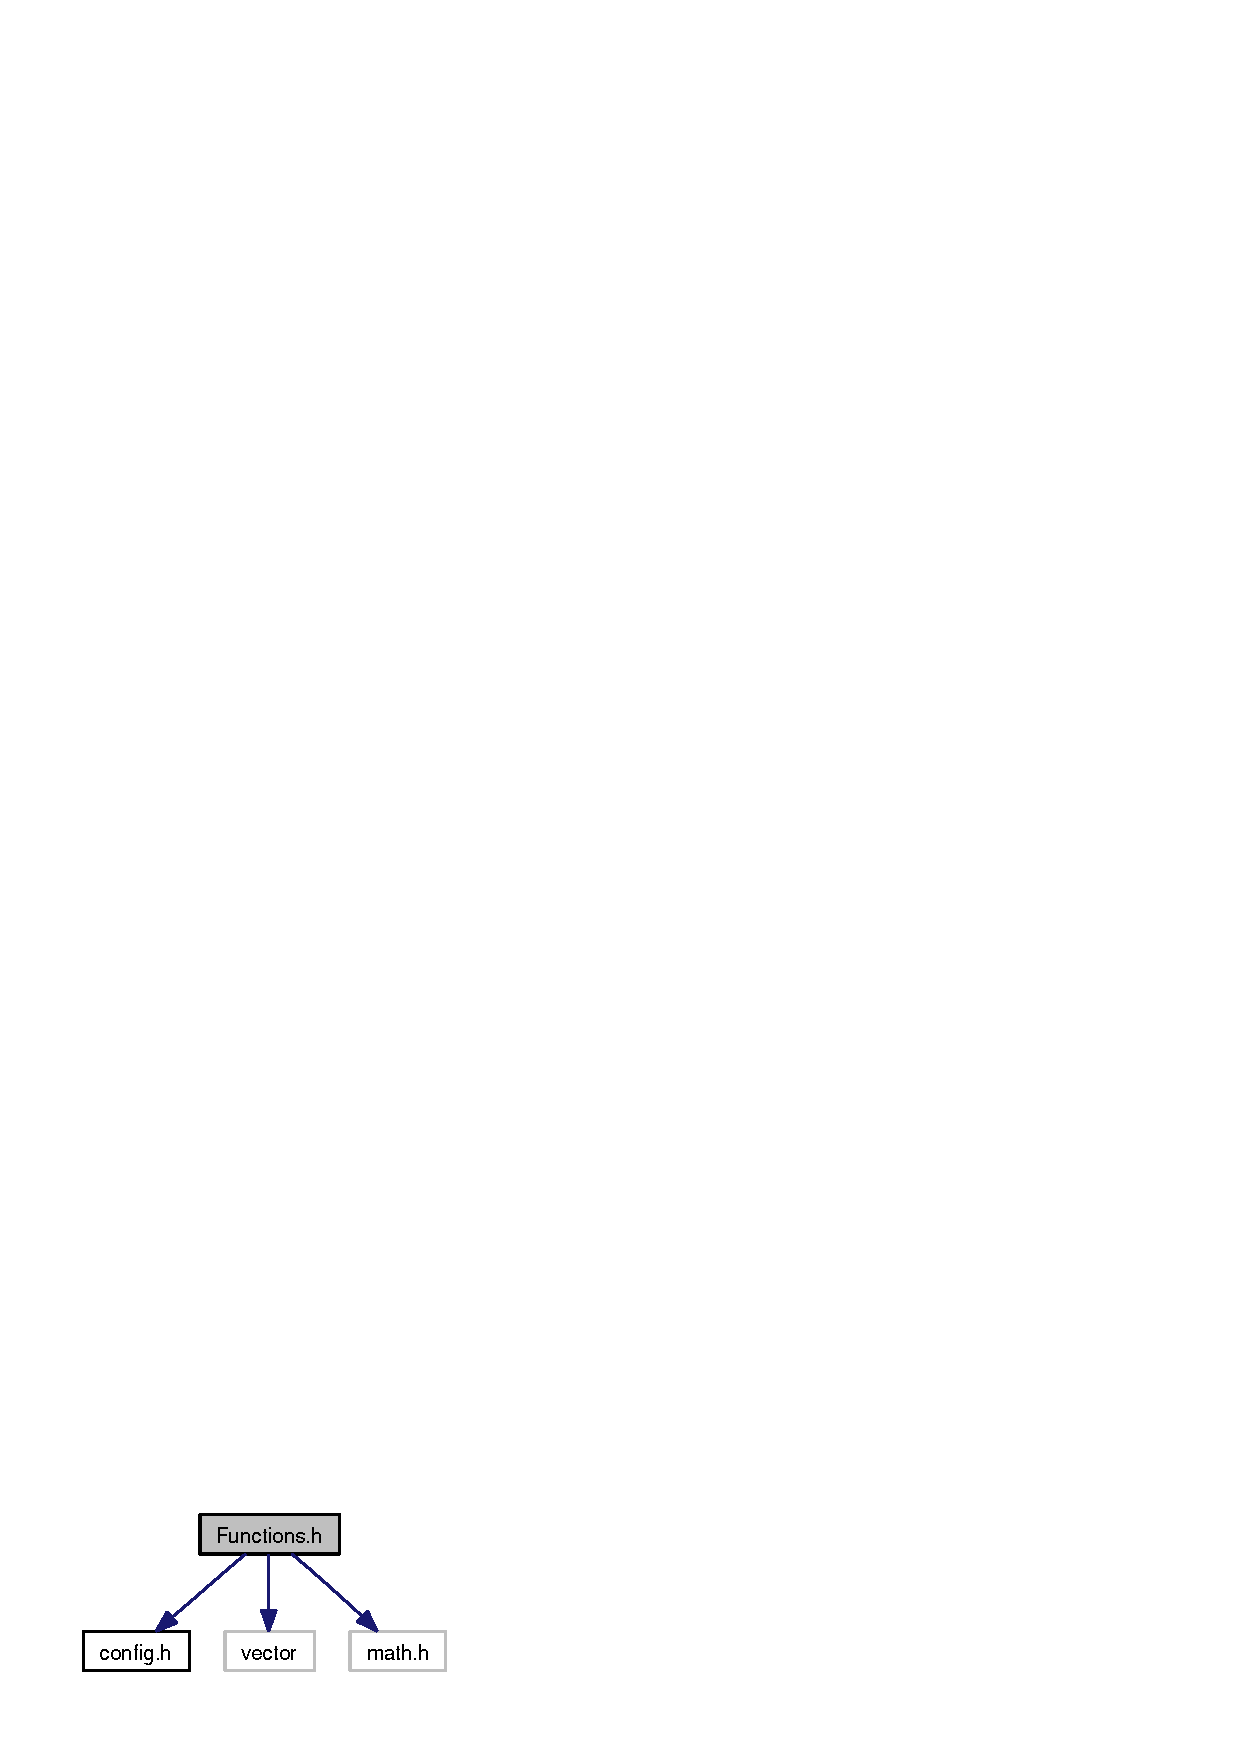
\includegraphics[width=109pt]{Functions_8h__incl}
\end{center}
\end{figure}


This graph shows which files directly or indirectly include this file:\nopagebreak
\begin{figure}[H]
\begin{center}
\leavevmode
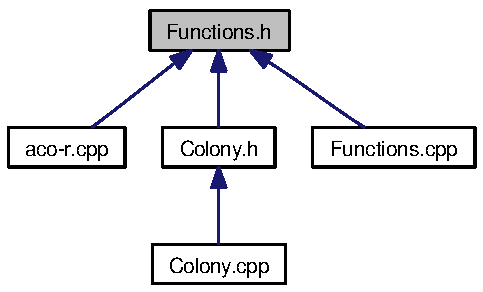
\includegraphics[width=134pt]{Functions_8h__dep__incl}
\end{center}
\end{figure}
\subsection*{Classes}
\begin{CompactItemize}
\item 
class \hyperlink{classFunction}{Function}
\item 
class \hyperlink{classGriewank}{Griewank}
\item 
class \hyperlink{classAckley}{Ackley}
\item 
class \hyperlink{classRastrigin}{Rastrigin}
\end{CompactItemize}

\hypertarget{Random_8cc}{
\section{Random.cc File Reference}
\label{Random_8cc}\index{Random.cc@{Random.cc}}
}
{\tt \#include \char`\"{}Random.h\char`\"{}}\par
{\tt \#include $<$stdio.h$>$}\par


Include dependency graph for Random.cc:\nopagebreak
\begin{figure}[H]
\begin{center}
\leavevmode
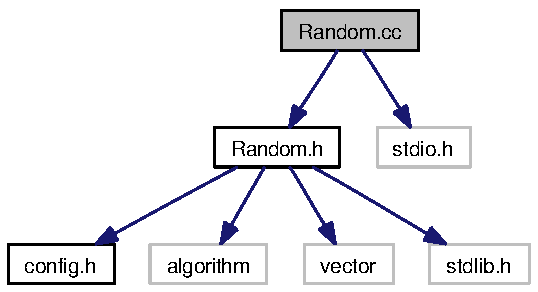
\includegraphics[width=147pt]{Random_8cc__incl}
\end{center}
\end{figure}
\subsection*{Defines}
\begin{CompactItemize}
\item 
\#define \hyperlink{Random_8cc_ce2e8e5cd08b605ab70bbf1a81185972}{VERBOSE}(x)~x
\item 
\#define \hyperlink{Random_8cc_61bdcb2fd2ebb805a31bde1ce782d732}{VERYVERBOSE}(x)
\end{CompactItemize}


\subsection{Define Documentation}
\hypertarget{Random_8cc_ce2e8e5cd08b605ab70bbf1a81185972}{
\index{Random.cc@{Random.cc}!VERBOSE@{VERBOSE}}
\index{VERBOSE@{VERBOSE}!Random.cc@{Random.cc}}
\subsubsection{\setlength{\rightskip}{0pt plus 5cm}\#define VERBOSE(x)~x}}
\label{Random_8cc_ce2e8e5cd08b605ab70bbf1a81185972}


\hypertarget{Random_8cc_61bdcb2fd2ebb805a31bde1ce782d732}{
\index{Random.cc@{Random.cc}!VERYVERBOSE@{VERYVERBOSE}}
\index{VERYVERBOSE@{VERYVERBOSE}!Random.cc@{Random.cc}}
\subsubsection{\setlength{\rightskip}{0pt plus 5cm}\#define VERYVERBOSE(x)}}
\label{Random_8cc_61bdcb2fd2ebb805a31bde1ce782d732}



\hypertarget{Random_8h}{
\section{Random.h File Reference}
\label{Random_8h}\index{Random.h@{Random.h}}
}
{\tt \#include \char`\"{}config.h\char`\"{}}\par
{\tt \#include $<$algorithm$>$}\par
{\tt \#include $<$vector$>$}\par
{\tt \#include $<$stdlib.h$>$}\par


Include dependency graph for Random.h:\nopagebreak
\begin{figure}[H]
\begin{center}
\leavevmode
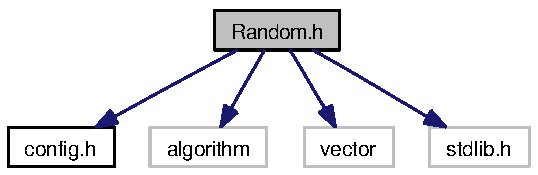
\includegraphics[width=147pt]{Random_8h__incl}
\end{center}
\end{figure}


This graph shows which files directly or indirectly include this file:\nopagebreak
\begin{figure}[H]
\begin{center}
\leavevmode
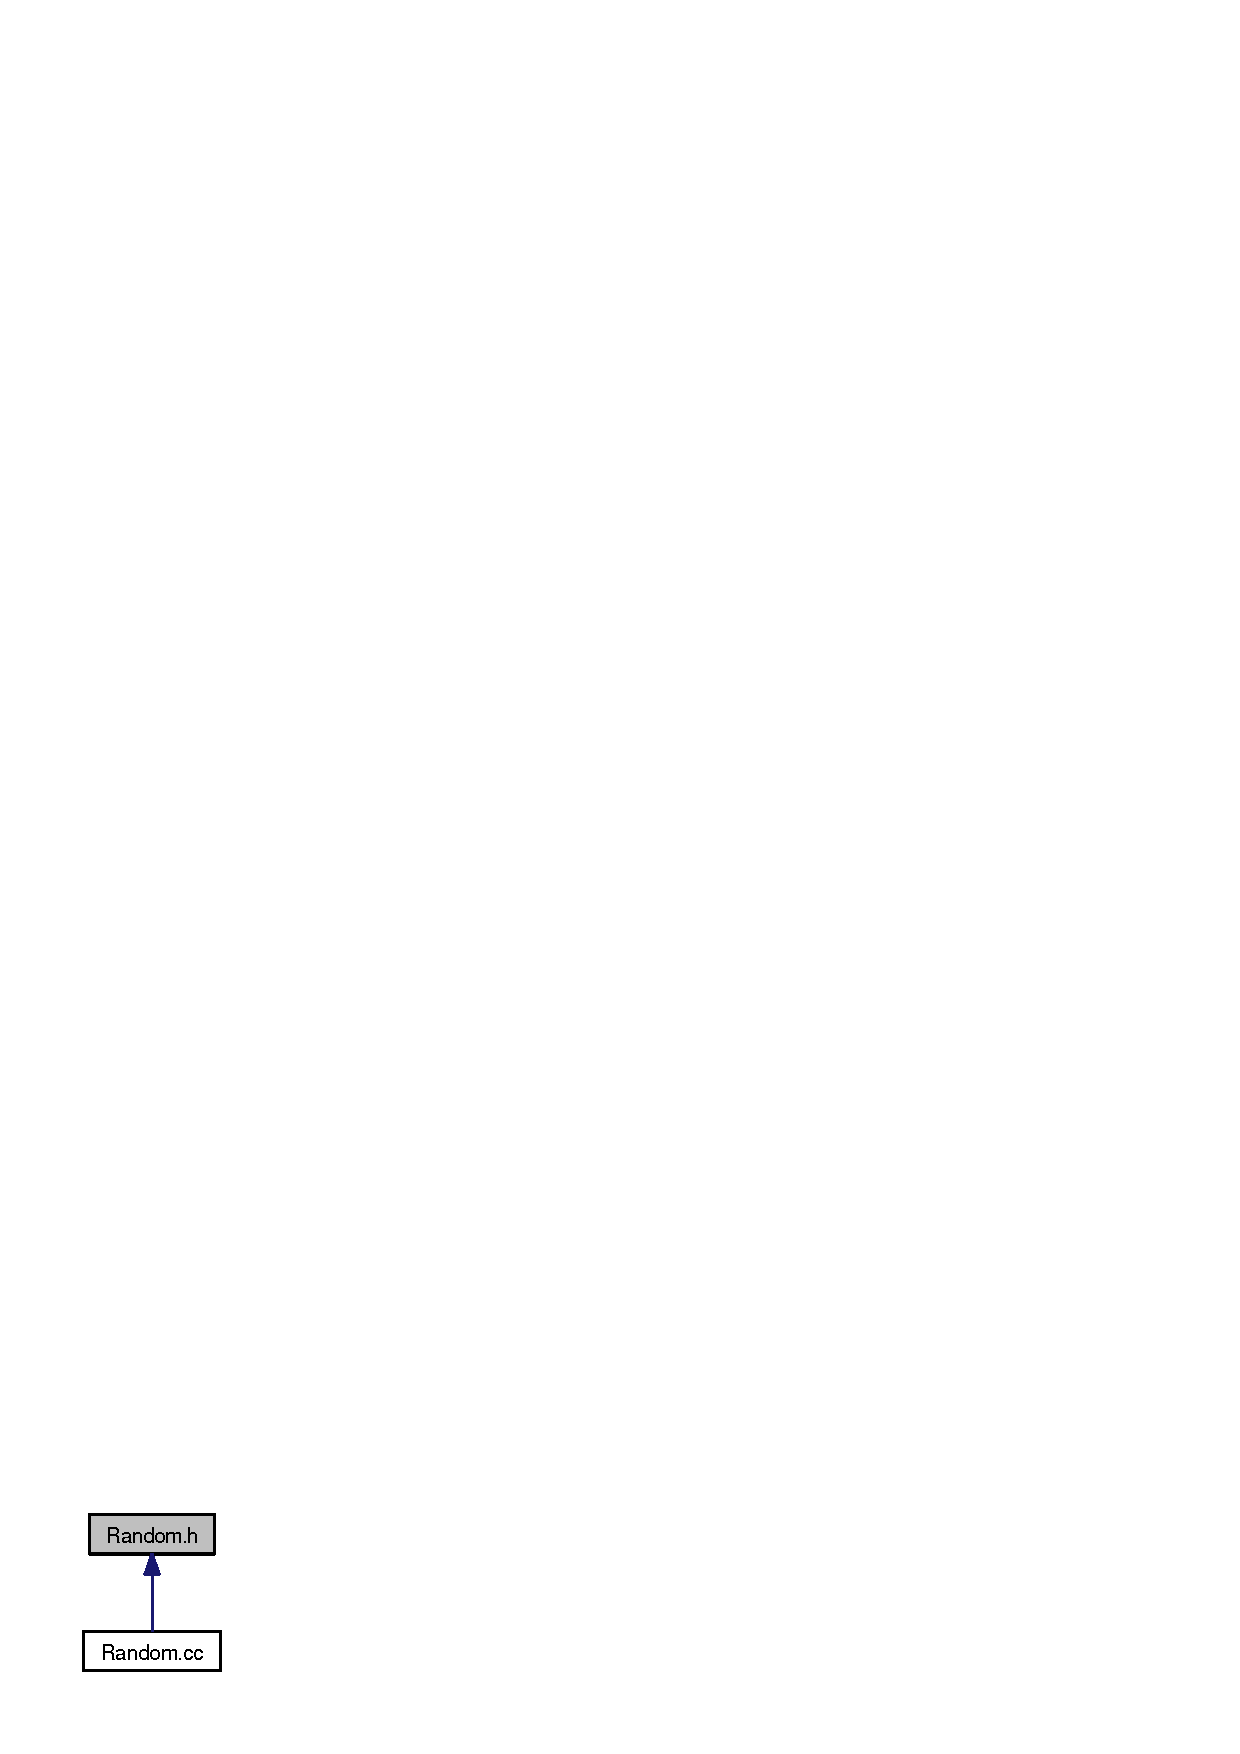
\includegraphics[width=55pt]{Random_8h__dep__incl}
\end{center}
\end{figure}
\subsection*{Classes}
\begin{CompactItemize}
\item 
class \hyperlink{classRandom}{Random}
\end{CompactItemize}

\hypertarget{Solution_8cpp}{
\section{Solution.cpp File Reference}
\label{Solution_8cpp}\index{Solution.cpp@{Solution.cpp}}
}
{\tt \#include \char`\"{}Solution.h\char`\"{}}\par


Include dependency graph for Solution.cpp:\nopagebreak
\begin{figure}[H]
\begin{center}
\leavevmode
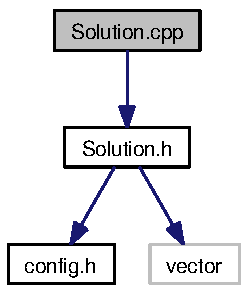
\includegraphics[width=77pt]{Solution_8cpp__incl}
\end{center}
\end{figure}

\hypertarget{Solution_8h}{
\section{Solution.h File Reference}
\label{Solution_8h}\index{Solution.h@{Solution.h}}
}
{\tt \#include \char`\"{}config.h\char`\"{}}\par
{\tt \#include $<$vector$>$}\par


Include dependency graph for Solution.h:\nopagebreak
\begin{figure}[H]
\begin{center}
\leavevmode
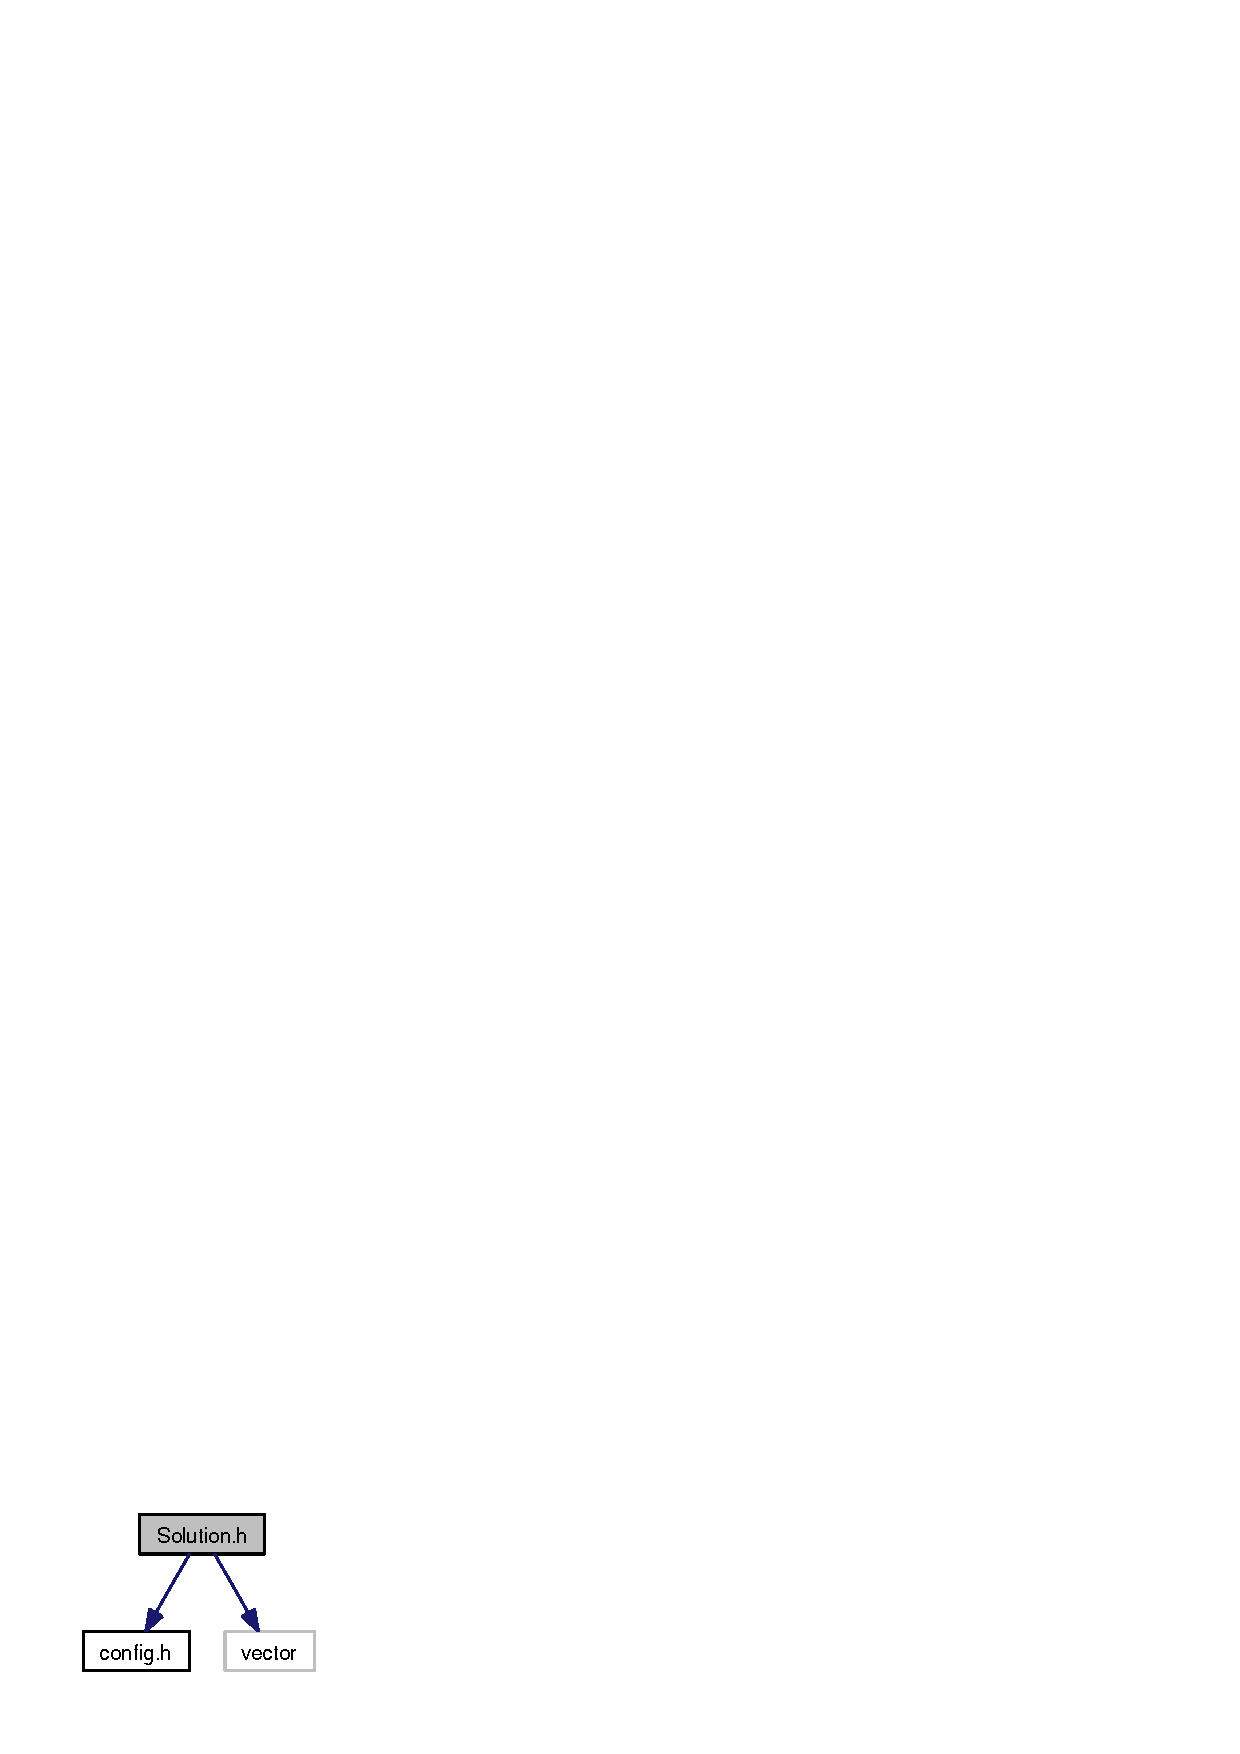
\includegraphics[width=77pt]{Solution_8h__incl}
\end{center}
\end{figure}


This graph shows which files directly or indirectly include this file:\nopagebreak
\begin{figure}[H]
\begin{center}
\leavevmode
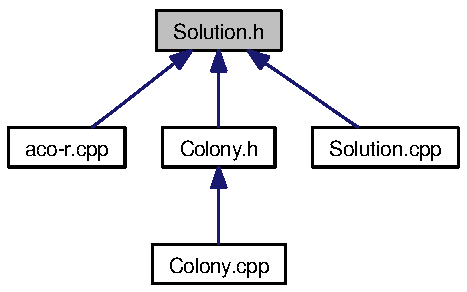
\includegraphics[width=130pt]{Solution_8h__dep__incl}
\end{center}
\end{figure}
\subsection*{Classes}
\begin{CompactItemize}
\item 
class \hyperlink{classSolution}{Solution}
\end{CompactItemize}

\hypertarget{Timer_8cc}{
\section{Timer.cc File Reference}
\label{Timer_8cc}\index{Timer.cc@{Timer.cc}}
}
{\tt \#include \char`\"{}Timer.h\char`\"{}}\par


Include dependency graph for Timer.cc:\nopagebreak
\begin{figure}[H]
\begin{center}
\leavevmode
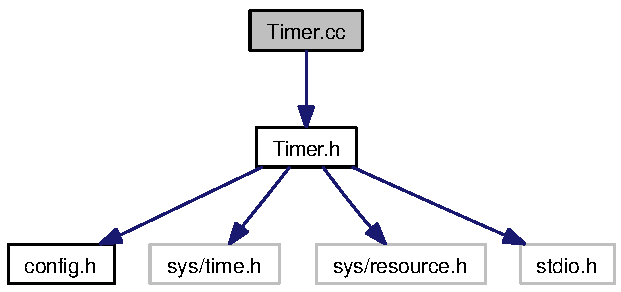
\includegraphics[width=167pt]{Timer_8cc__incl}
\end{center}
\end{figure}

\hypertarget{Timer_8h}{
\section{Timer.h File Reference}
\label{Timer_8h}\index{Timer.h@{Timer.h}}
}
{\tt \#include \char`\"{}config.h\char`\"{}}\par
{\tt \#include $<$sys/time.h$>$}\par
{\tt \#include $<$sys/resource.h$>$}\par
{\tt \#include $<$stdio.h$>$}\par


Include dependency graph for Timer.h:\nopagebreak
\begin{figure}[H]
\begin{center}
\leavevmode
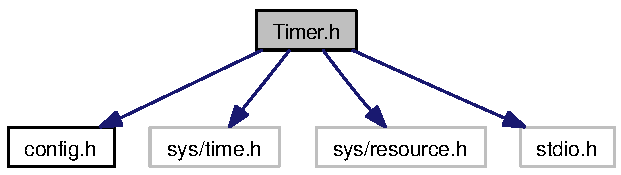
\includegraphics[width=167pt]{Timer_8h__incl}
\end{center}
\end{figure}


This graph shows which files directly or indirectly include this file:\nopagebreak
\begin{figure}[H]
\begin{center}
\leavevmode
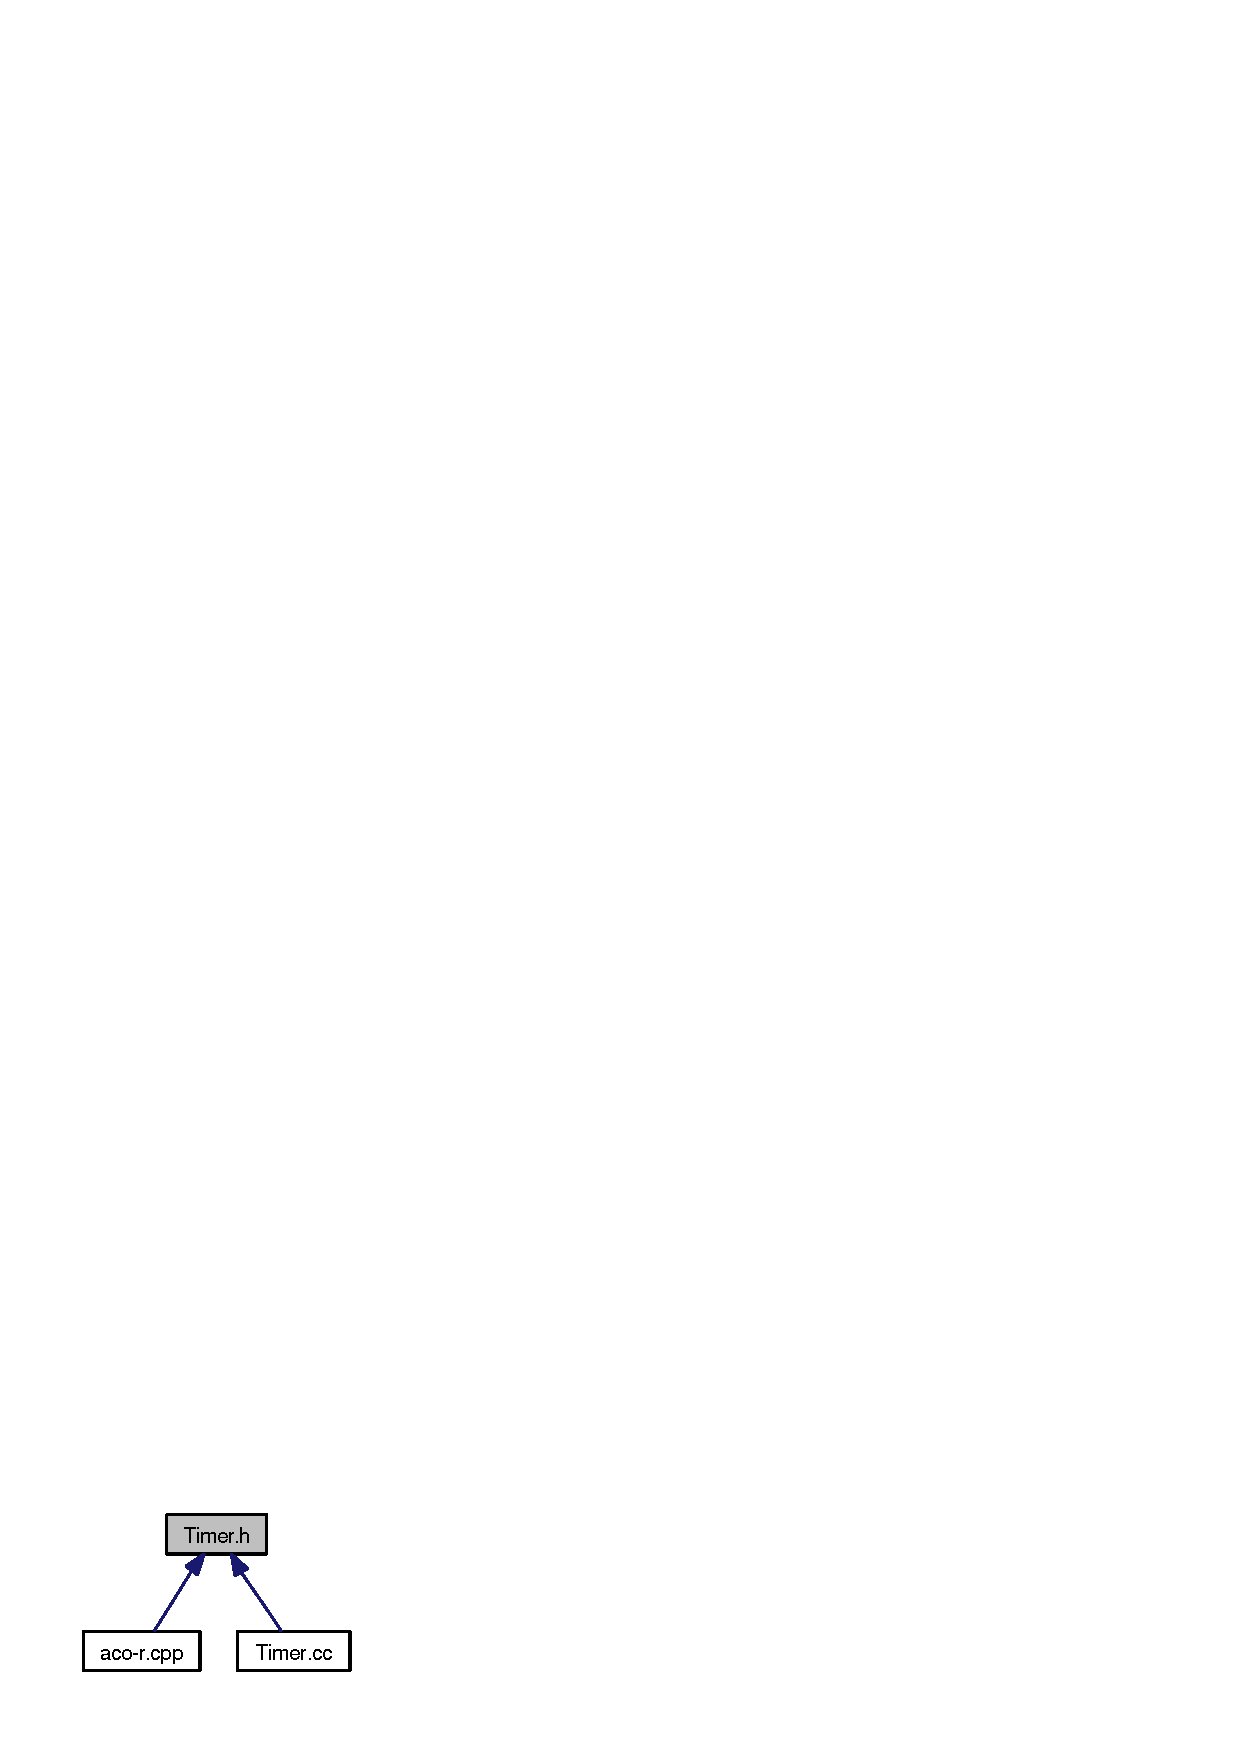
\includegraphics[width=86pt]{Timer_8h__dep__incl}
\end{center}
\end{figure}
\subsection*{Classes}
\begin{CompactItemize}
\item 
class \hyperlink{classTimer}{Timer}
\end{CompactItemize}

\printindex
\end{document}
